\documentclass[11pt,a4paper]{report}

\usepackage[T1]{fontenc}
\usepackage[utf8]{inputenc}
\usepackage{lmodern}
\usepackage[margin=1in]{geometry}
\usepackage{xcolor}
\usepackage{tikz}
\usetikzlibrary{arrows.meta,positioning,shapes.geometric,fit,calc,backgrounds,decorations.pathreplacing}
\usepackage{booktabs}
\usepackage{longtable}
\usepackage{array}
\newcolumntype{L}[1]{>{\raggedright\arraybackslash}p{#1}}
\usepackage{listings}
\usepackage{amsmath}
\usepackage{siunitx}
\usepackage{float}
\usepackage{enumitem}
\usepackage{caption}
\usepackage{fancyhdr}
\usepackage[hidelinks,pdfusetitle,plainpages=false,pdfpagelabels]{hyperref}
\urlstyle{tt}

% ---------------------------------------------------------------- colours
% One colour family for deterministic code, one for steps that touch the language model, grey for everything else.
\definecolor{detline}{RGB}{31,78,121}
\definecolor{detfill}{RGB}{221,235,247}
\definecolor{llmline}{RGB}{196,89,17}
\definecolor{llmfill}{RGB}{253,230,200}
\definecolor{neuline}{RGB}{89,89,89}
\definecolor{neufill}{RGB}{238,238,238}
\definecolor{outline}{RGB}{60,60,60}

% ---------------------------------------------------------------- macros
% \code{} prints verbatim-like identifiers (underscores, %, #, & are safe); \fpath{} breaks long paths at slashes.
% breakable code: characters are typeset literally, with a break opportunity after _ / . : , ; =
\ExplSyntaxOn
\NewDocumentCommand{\code}{m}{\texttt{\str_map_inline:nn{#1}{\__sdcv_char:n{##1}}}}
\cs_new:Npn \__sdcv_char:n #1 { #1 \str_case:nnF {#1} { {_}{\allowbreak} {/}{\allowbreak} {.}{\allowbreak} {:}{\allowbreak} {,}{\allowbreak} {;}{\allowbreak} {=}{\allowbreak} } {} }
\ExplSyntaxOff
\DeclareRobustCommand{\fpath}[1]{\path{#1}}
\newcommand{\clause}[1]{Cl.~#1}
\newcommand{\sdcv}{SDC-V}
\newcommand{\stamp}{DRAFT: requires review and sign-off by a licensed structural engineer. This output is not a certified design.}
\newcommand{\detkey}{\tikz[baseline=-0.6ex]\node[draw=detline,fill=detfill,rounded corners=1pt,minimum width=6mm,minimum height=3mm,inner sep=0pt]{};}
\newcommand{\llmkey}{\tikz[baseline=-0.6ex]\node[draw=llmline,fill=llmfill,rounded corners=1pt,minimum width=6mm,minimum height=3mm,inner sep=0pt]{};}
\newcommand{\neukey}{\tikz[baseline=-0.6ex]\node[draw=neuline,fill=neufill,rounded corners=1pt,minimum width=6mm,minimum height=3mm,inner sep=0pt]{};}

% shared TikZ styles
\tikzset{
  det/.style={draw=detline,fill=detfill,rounded corners=2pt,align=center,font=\small,inner sep=4pt,minimum height=7mm},
  llm/.style={draw=llmline,fill=llmfill,rounded corners=2pt,align=center,font=\small,inner sep=4pt,minimum height=7mm},
  neu/.style={draw=neuline,fill=neufill,rounded corners=2pt,align=center,font=\small,inner sep=4pt,minimum height=7mm},
  flow/.style={-{Stealth[length=2.2mm]},thick,color=outline},
  flowd/.style={-{Stealth[length=2.2mm]},thick,color=outline,dashed},
  lbl/.style={font=\scriptsize,color=outline,inner sep=1.5pt},
}

% ---------------------------------------------------------------- listings
\lstset{
  basicstyle=\ttfamily\footnotesize,
  breaklines=true,
  breakatwhitespace=false,
  columns=fullflexible,
  keepspaces=true,
  frame=single,
  rulecolor=\color{neuline},
  backgroundcolor=\color{neufill!40},
  aboveskip=8pt,
  belowskip=8pt,
  xleftmargin=4pt,
  xrightmargin=4pt,
  showstringspaces=false,
}

% ---------------------------------------------------------------- layout
\setlength{\headheight}{14pt}
\setlength{\parindent}{0pt}
\setlength{\parskip}{0.55\baselineskip}
\renewcommand{\arraystretch}{1.12}
\captionsetup{font=small,labelfont=bf,skip=6pt}
\setlist{itemsep=2pt,topsep=3pt,parsep=0pt}
\emergencystretch=2em

\pagestyle{fancy}
\fancyhf{}
\fancyhead[L]{\small\textbf{DRAFT: not a certified design}}
\fancyhead[R]{\small SDC-V 0.2.0 technical report}
\fancyfoot[C]{\small\thepage}
\renewcommand{\headrulewidth}{0.4pt}
\fancypagestyle{plain}{%
  \fancyhf{}%
  \fancyhead[L]{\small\textbf{DRAFT: not a certified design}}%
  \fancyhead[R]{\small SDC-V 0.2.0 technical report}%
  \fancyfoot[C]{\small\thepage}%
  \renewcommand{\headrulewidth}{0.4pt}}

\hypersetup{pdftitle={SDC-V: Structural Design Copilot with Deterministic Verifier. Technical Report},
            pdfsubject={SDC-V version 0.2.0, IS 456:2000},
            pdfkeywords={IS 456:2000, reinforced concrete beam, deterministic verifier, LLM guardrails}}

\begin{document}

% ================================================================ title page
\begin{titlepage}
\thispagestyle{empty}
\centering
\vspace*{2.2cm}
{\Huge\bfseries SDC-V\par}
\vspace{0.5cm}
{\LARGE Structural Design Copilot\\[2pt] with Deterministic Verifier\par}
\vspace{1.0cm}
{\Large Technical Report\par}
\vspace{2.0cm}
\begin{tabular}{@{}ll@{}}
\toprule
Software version & 0.2.0 \\
Code edition     & IS 456:2000 \\
Report date      & 15 November 2026 \\
Subject          & Singly reinforced rectangular RCC beams, limit state method \\
\bottomrule
\end{tabular}
\vfill
\fbox{\parbox{0.86\textwidth}{\centering\small\textbf{\stamp}}}
\vspace{1.0cm}
\end{titlepage}

\pagenumbering{roman}
\setcounter{page}{2}

% ================================================================ front matter
\chapter*{Abstract}
\addcontentsline{toc}{chapter}{Abstract}

\sdcv{} (Structural Design Copilot with Deterministic Verifier) is a web application and JSON API that produces a draft design of a singly reinforced rectangular reinforced-concrete beam to IS~456:2000~\cite{is456}. The input is either a structured form or a plain-English brief. A language model, the Google Gemini API~\cite{gemini}, is used at two points only: to extract fields from the brief, and to write the explanatory text of a result that has already been computed and verified. Every engineering number is produced by a deterministic Python calculator. Every pass or fail verdict is produced by a registry of 19 clause-tagged rules, two of which are independent cross-checks of the calculator. When an error-level rule that resizing can fix fails, a deterministic reviser enlarges the section in 25~mm steps, depth first and then width. Model-written text is accepted only if every number in it appears in the verified result; after three rejected attempts a deterministic template is used.

This report documents the scope, architecture, design method, verification layer, guardrails, data flow, API, audit database, browser interface, test and benchmark programme, deployment and security posture, limitations and possible future work of version 0.2.0. Statements were checked against the source code of the repository, and where the project README and the code disagree the code is followed. Counts quoted in the text (19 rules, 105 knowledge-base entries in 19 topics, a 51-section explorer, a 60-case end-to-end benchmark) were reproduced by running the code. The test suite, the benchmark and the worked examples in Appendix~\ref{app:example} were executed while this report was prepared. All output of the tool is a draft and requires review by a licensed structural engineer.


\tableofcontents
\listoffigures
\listoftables

\clearpage
\pagenumbering{arabic}

% ================================================================ body
\chapter{Introduction and problem statement}\label{ch:intro}

\section{Problem}
Drafting a singly reinforced rectangular beam by hand involves a long chain of small calculations: loads, bending moment and shear force, flexural reinforcement, bar selection, shear reinforcement, deflection control and detailing rules. A single wrong number is difficult to spot in such a chain, and the cost of an unnoticed error is a member that is under-designed. A language model is attractive as a front end, because engineers describe beams in words, sketches and tender extracts rather than in the fields of a form. It is unsuitable as a calculator.

\section{Why a language model must never own a number}
A language model produces text that is statistically plausible. It does not execute the formulae of a design code, and it can state a value that looks right but is wrong, with no indication of the error. For structural design this property is unacceptable in three specific ways.
\begin{enumerate}
  \item \textbf{Silent numerical errors.} An arithmetic slip, a wrong table lookup or a mixed-up unit in generated text is indistinguishable from a correct value.
  \item \textbf{No stable verdict.} The same prompt can yield different numbers on different occasions, so a result cannot be reproduced, audited or tested against reference values.
  \item \textbf{Susceptibility to instructions in the data.} A pasted specification or an image can contain text that tries to steer the model, for example to approve a design or to relax a margin.
\end{enumerate}
\sdcv{} therefore separates the two concerns. Code owns every number and every verdict. The model is confined to reading the brief and to narrating a result that has already been verified, and its narrative is checked mechanically against that result. This is the central design rule of the project, and the remaining chapters follow from it: the \emph{trust boundary} lies between the model and the numbers.

\section{Objectives}
The system is intended to:
\begin{itemize}
  \item produce a checked first draft of a beam section and its reinforcement for a supported class of beams, using the limit state method of IS~456:2000;
  \item accept input from a structured form and from natural language, with optional images and a pasted attachment;
  \item verify every result with rules that cite a clause of the code, including two independent recomputations of key quantities;
  \item record every run in an audit log with the code edition, a fingerprint of the rule set and the tool versions;
  \item reject, rather than approximate, anything outside its scope, and refuse requests to approve, certify or relax safety requirements.
\end{itemize}

\section{Intended users and status of the output}
Intended users are structural engineers and students who want a fast, checked first draft, and developers who want a reference for a guarded language-model pipeline in which the model never owns a number. The tool does not replace engineering judgement. All output carries the stamp
\begin{quote}\small\textbf{\stamp}\end{quote}
which is a constant in the code (\code{STAMP} in \fpath{backend/app/report.py}); the narrative is rejected by the output guardrail if the model omits it.

\section{Organisation of this report}
Chapter~\ref{ch:scope} defines the scope. Chapters~\ref{ch:arch} to~\ref{ch:llm} describe the architecture, the design method, the verification layer and the model integration. Chapters~\ref{ch:flow} to~\ref{ch:frontend} describe the data flow, the API, the audit database and the browser interface. Chapters~\ref{ch:test} to~\ref{ch:perf} cover testing, deployment, security and performance. Chapters~\ref{ch:limits} to~\ref{ch:concl} give the limitations, a roadmap and the conclusion. Appendices list the environment variables, the directory tree and worked design examples.

\chapter{Scope and system boundaries}\label{ch:scope}

The supported scope is enforced in code, not by documentation. The limits below are the constraints of the \code{BeamInput} model in \fpath{backend/app/schemas.py}; the scope view of the interface and \code{GET /api/scope} read the same constraints, so the description cannot drift from the validation.

\section{In-scope design problem}
\sdcv{} designs singly reinforced rectangular beams, simply supported or cantilever, under a uniformly distributed load, by the limit state method of IS~456:2000.

\begin{table}[H]
\centering
\caption{Accepted input ranges (\code{BeamInput}). The model also applies the cross-field rules listed below the table.}
\label{tab:ranges}
\begin{tabular}{@{}L{4.9cm}L{4.4cm}L{5.4cm}@{}}
\toprule
Quantity & Range or values & Notes \\
\midrule
Effective span $L$ (\code{span_m}) & $0 < L \le 15$ m & Cantilever length at most 6 m \\
Width $b$ (\code{b_mm}) & 150 to 1000 mm & \\
Overall depth $D$ (\code{D_mm}) & 200 to 2000 mm & $D/b \le 4$ \\
Nominal cover & 20 to 100 mm & At least 100 mm less than $D$ \\
Concrete grade $f_{ck}$ & M20, M25, M30, M35, M40 & Stored as 20 to 40 \\
Steel grade $f_y$ & Fe250, Fe415, Fe500 & Stored as 250, 415, 500 \\
Exposure & mild, moderate, severe, very severe, extreme & \\
Support & simply supported, cantilever & \\
Superimposed dead load & 0 to 500 kN/m & Excludes self-weight \\
Live load & 0 to 500 kN/m & Dead plus live must be greater than zero \\
\bottomrule
\end{tabular}
\end{table}

The cross-field rules of the model are: $D/b \le 4$; a cantilever length of at most 6~m; dead plus live load greater than zero; and $D \ge \text{cover} + 100$~mm. Input may be given in other units; the normaliser converts lengths in mm, cm, m, in and ft, and line loads in kN/m, N/mm, N/m, t/m, kgf/m, lb/ft and kip/ft, and records each conversion. Area loads (for example kN/m$^2$) and point forces are rejected with an explanation, because a line load per metre of beam is required.

\section{Declined features}
The scope screen (Chapter~\ref{ch:llm}) detects the following features in the user's words and returns the status \code{out_of_scope}. Nothing is approximated.
\begin{itemize}
  \item flanged sections (T and L beams);
  \item doubly reinforced beams;
  \item continuous beams (two-span, multi-span);
  \item slabs, columns, footings and foundations;
  \item prestressed concrete;
  \item design codes other than IS~456:2000 (for example Eurocode~2, ACI, AS~3600, BS~8110);
  \item seismic and ductile detailing (IS~13920);
  \item steel design (IS~800);
  \item walls, retaining structures and deep beams;
  \item point and concentrated loads.
\end{itemize}
Continuous, fixed or propped support conditions given as a support value are also declined by the normaliser.

\section{Refused unsafe requests}
Four classes of request return the status \code{refused} and no model is called: approving or certifying a design; reducing safety margins; removing structural elements; and skipping inspections. Mentions that merely use similar words in ordinary engineering language (for example ``approved drawings'') do not trigger the refusal, and a negated mention (for example ``not a T-beam'') does not trigger a decline.

\section{Not provided}
The repository does not provide user accounts, roles, multi-tenant isolation, a Docker or CI configuration, or a licence file. These are discussed in Chapters~\ref{ch:deploy} and~\ref{ch:limits}.

\chapter{System architecture}\label{ch:arch}

\section{Four layers}
The system has four layers, shown in Figure~\ref{fig:arch}.
\begin{enumerate}
  \item \textbf{Browser interface.} Static HTML, CSS and native ES modules in \fpath{frontend/}, with no build step and no third-party runtime dependency.
  \item \textbf{Optional Node proxy.} \fpath{frontend/server.mjs} serves the static files and forwards \code{/api/*} to the backend. The backend can also serve the interface itself.
  \item \textbf{FastAPI backend.} \fpath{backend/app/} is a JSON API plus a static file server~\cite{fastapi}, served by Uvicorn~\cite{uvicorn} and using Pydantic models~\cite{pydantic} at its boundaries. A request middleware performs the token check, the rate limit, the security headers and the request log.
  \item \textbf{Persistence and external services.} A SQLite audit log~\cite{sqlite} in \fpath{backend/data/audit.db}, and the Google Gemini REST API~\cite{gemini}, which is the only external service.
\end{enumerate}

\begin{figure}[H]
\centering
% High-level four-layer architecture. Styles det, llm, neu and flow come from main.tex.
{\hyphenpenalty=10000\exhyphenpenalty=10000
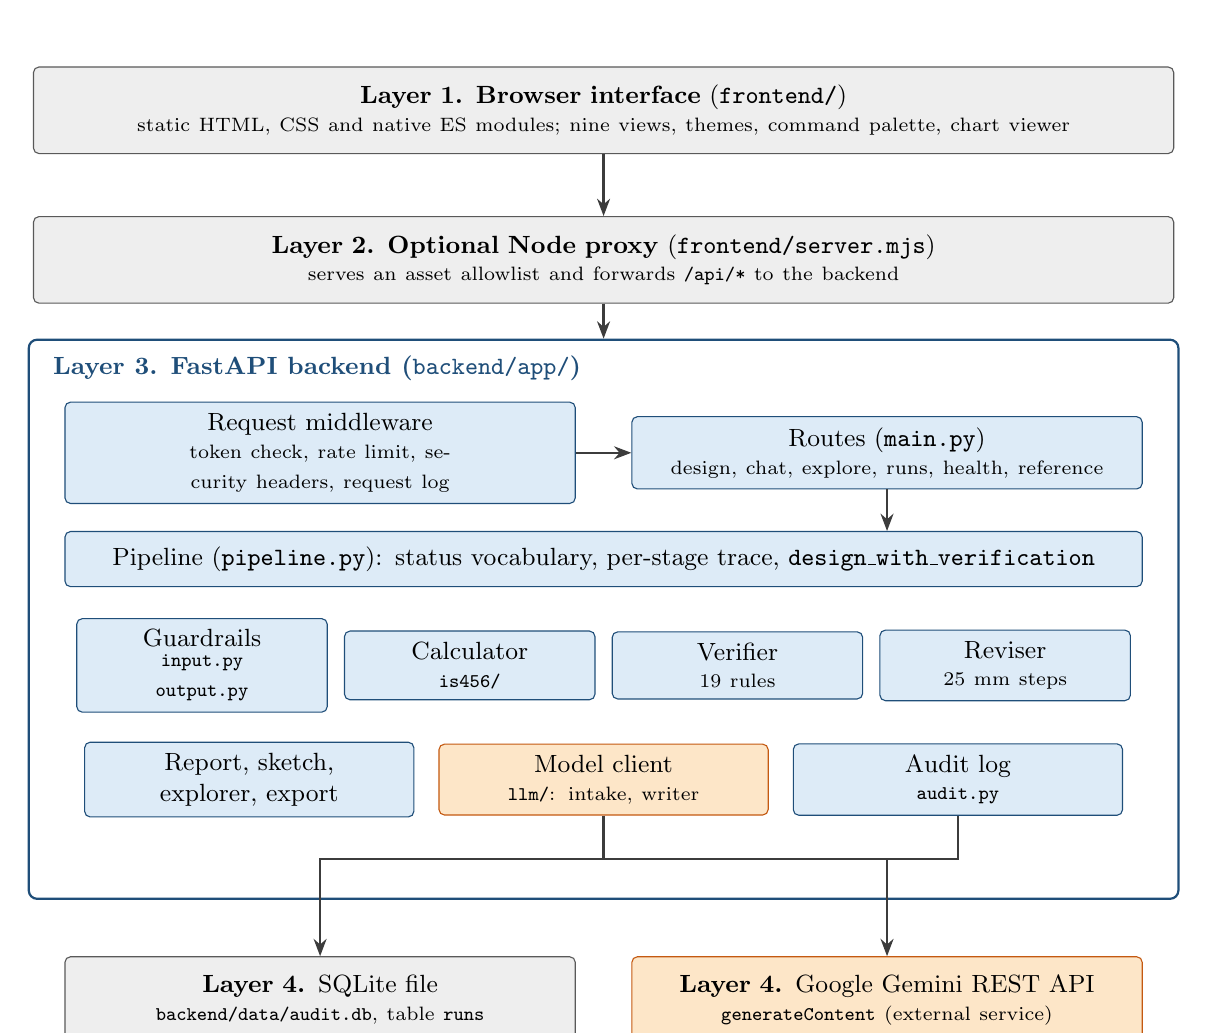
\begin{tikzpicture}[x=1cm,y=1cm]
  % layer 1: browser
  \node[neu,text width=14.2cm,minimum height=1.1cm] (l1) at (0,0)
    {\textbf{Layer 1. Browser interface} (\texttt{frontend/})\\[-1pt]\scriptsize static HTML, CSS and native ES modules; nine views, themes, command palette, chart viewer};
  % layer 2: proxy
  \node[neu,text width=14.2cm,minimum height=1.1cm] (l2) at (0,-1.9)
    {\textbf{Layer 2. Optional Node proxy} (\texttt{frontend/server.mjs})\\[-1pt]\scriptsize serves an asset allowlist and forwards \texttt{/api/*} to the backend};
  % layer 3: backend container
  \node[draw=detline,rounded corners=3pt,thick,minimum width=14.6cm,minimum height=7.1cm,anchor=north] (l3) at (0,-2.9) {};
  \node[font=\small\bfseries,anchor=north west,text=detline] at ($(l3.north west)+(0.2,-0.1)$) {Layer 3. FastAPI backend (\texttt{backend/app/})};
  \node[det,text width=6.2cm] (mw) at (-3.6,-4.35) {Request middleware\\[-1pt]\scriptsize token check, rate limit, security headers, request log};
  \node[det,text width=6.2cm] (rt) at (3.6,-4.35) {Routes (\texttt{main.py})\\[-1pt]\scriptsize design, chat, explore, runs, health, reference};
  \node[det,text width=13.4cm] (pl) at (0,-5.7) {Pipeline (\texttt{pipeline.py}): status vocabulary, per-stage trace, \texttt{design\_with\_verification}};
  \node[det,text width=2.9cm] (gr) at (-5.1,-7.05) {Guardrails\\[-1pt]\scriptsize\texttt{input.py}\\\texttt{output.py}};
  \node[det,text width=2.9cm] (ca) at (-1.7,-7.05) {Calculator\\[-1pt]\scriptsize\texttt{is456/}};
  \node[det,text width=2.9cm] (ve) at (1.7,-7.05) {Verifier\\[-1pt]\scriptsize 19 rules};
  \node[det,text width=2.9cm] (re) at (5.1,-7.05) {Reviser\\[-1pt]\scriptsize 25 mm steps};
  \node[det,text width=3.9cm] (rp) at (-4.5,-8.5) {Report, sketch, explorer, export};
  \node[llm,text width=3.9cm] (lc) at (0,-8.5) {Model client\\[-1pt]\scriptsize\texttt{llm/}: intake, writer};
  \node[det,text width=3.9cm] (au) at (4.5,-8.5) {Audit log\\[-1pt]\scriptsize\texttt{audit.py}};
  % layer 4
  \node[neu,text width=6.2cm,minimum height=1.1cm] (db) at (-3.6,-11.3) {\textbf{Layer 4.} SQLite file\\[-1pt]\scriptsize\texttt{backend/data/audit.db}, table \texttt{runs}};
  \node[llm,text width=6.2cm,minimum height=1.1cm] (gm) at (3.6,-11.3) {\textbf{Layer 4.} Google Gemini REST API\\[-1pt]\scriptsize \texttt{generateContent} (external service)};
  % arrows
  \draw[flow] (l1) -- (l2);
  \draw[flow] (l2) -- ($(l3.north)+(0,0)$);
  \draw[flow] (au.south) -- ++(0,-0.55) -| (db.north);
  \draw[flow] (lc.south) -- ++(0,-0.55) -| (gm.north);
  \draw[flow] (mw.east) -- (rt.west);
  \draw[flow] (rt.south) -- (rt.south |- pl.north);
\end{tikzpicture}}

\vspace{4pt}
{\small\detkey{} deterministic code \quad \llmkey{} touches the language model \quad \neukey{} browser, proxy, storage}

\caption{High-level four-layer architecture. Blue marks deterministic code, orange marks the only module that talks to the language model, grey marks the browser, proxy and storage.}
\label{fig:arch}
\end{figure}

\section{Backend modules}
One \code{AuditLog}, one \code{GeminiClient}, one \code{Pipeline} and one \code{RateLimiter} are instantiated at import time in \code{main.py}. Each request that needs the pipeline calls \code{pipeline.with_model(model)}, which returns a new \code{Pipeline} bound to a per-request \code{GeminiClient} that tries the selected model first and then the other configured models. Per-request state (trace, attempts, last model) is therefore never shared between requests. Table~\ref{tab:modules} lists the modules.

\begin{longtable}{@{}L{4.3cm}L{10.7cm}@{}}
\caption{Backend modules in \fpath{backend/app/}. Line counts are not given because they change with every edit.}\label{tab:modules}\\
\toprule Module & Responsibility \\ \midrule \endfirsthead
\toprule Module & Responsibility \\ \midrule \endhead
\bottomrule \endlastfoot
\code{main.py} & FastAPI application, request and response models, the request middleware, all routes and the static file routes (\code{/} and \code{/static/{name}}); configures logging. \\
\code{config.py} & Loads \code{.env} files; defines the model list, timeouts, rate limit, API token accessor, data directory and the reviser and writer limits. Holds \code{APP_VERSION} (``0.2.0''). \\
\code{pipeline.py} & Orchestrator. Owns the status vocabulary, the verification loop \code{design_with_verification}, the \code{RunResult} response model, the per-stage trace and \code{tool_versions}. \\
\code{schemas.py} & Pydantic models: \code{BeamInput}, \code{CheckResult}, \code{BarArrangement}, \code{Design}. \\
\code{is456/calculator.py} & \code{design_beam}: the deterministic calculator. Pure Python, no I/O. \\
\code{is456/tables.py} & IS~456:2000 constants and tables with clause references, and the fitted functions \code{tau_c} and \code{deflection_modification}. \\
\code{verifier.py} & The rule registry: 19 rules registered with the \code{@rule} decorator, \code{RULE_META}, \code{run_rules} and \code{rules_fingerprint}. \\
\code{reviser.py} & Deterministic section reviser. \\
\code{guardrails/input.py} & \code{RawIntake}, unit normalisation, range validation, scope and unsafe-request screening, injection flags, PII redaction, number extraction for grounding. \\
\code{guardrails/output.py} & \code{trace_numbers}: the number-trace output guardrail. \\
\code{llm/gemini.py} & \code{GeminiClient}, the \code{LLM} protocol, \code{LLMError}, \code{parse_json}. \\
\code{llm/intake.py} & The intake agent: system prompt and \code{run_intake}. \\
\code{llm/writer.py} & The writer prompt and \code{write_report}. \\
\code{llm/vision.py}, \code{llm/local.py}, \code{llm/factory.py} & Optional two-stage intake: a vision transcriber and optional local models, enabled only through \code{SDCV_*} settings. \\
\code{report.py} & \code{ReportData} (pre-formatted strings), the draft \code{STAMP}, \code{build_report_data}, the template narrative. \\
\code{sketch.py} & Server-side SVG cross-section for reports and exports. \\
\code{explore.py} & The what-if section explorer. No model, no audit write. \\
\code{export.py} & Markdown report of a stored run and CSV export with spreadsheet formula-injection protection. \\
\code{scope.py} & Builds the supported-scope description from \code{BeamInput} and the guard pattern labels. \\
\code{security.py} & Client address resolution, sliding-window \code{RateLimiter}, constant-time token comparison, security headers. \\
\code{audit.py} & The SQLite audit log. \\
\code{kb.py} & The reference knowledge base: 105 entries in 19 topics. \\
\code{system_model.py} & Describes the system as a knowledge-based system (facts, derivation rules, verifier rules, guardrail rules, meta-rules, modules, endpoints). \\
\end{longtable}

\section{Design patterns}
\begin{itemize}
  \item \textbf{Pipeline with explicit stages and a status vocabulary} (\code{designed}, \code{needs_engineer}, \code{needs_info}, \code{rejected}, \code{out_of_scope}, \code{refused}, \code{error}).
  \item \textbf{Rule registry.} Rules are plain functions registered with a decorator, which gives a single source for the verifier, the rule-list endpoint and the rule fingerprint.
  \item \textbf{Protocol-based model client.} The \code{LLM} protocol (\code{generate(system, user, json_mode, images)}) is the only contract the pipeline needs, which is how tests substitute a scripted fake.
  \item \textbf{Fail closed.} If the model is unavailable, unparseable or untraceable, the result is an explicit error status or a deterministic template, never a guessed value.
  \item \textbf{Allowlists over blocklists} for static files and model identifiers.
  \item \textbf{Single source of truth for scope}, as described in Chapter~\ref{ch:scope}.
\end{itemize}

\section{Frontend modules}
The interface is vanilla JavaScript loaded as native ES modules from \code{app.js}. \code{chrome.js} owns the shell (header, sidebar, router, status bar, command palette, theme). Each view is one module that registers itself with the router; \code{result.js} renders a design result for the form, history and assistant views. \code{theme.css} is the only place colours are defined: deterministic output (calculator, verifier, reviser, audit) is coloured differently from language-model output (intake, narrative), and green, amber and red are reserved for verdicts. Beam drawings in \code{beam.js} are inline SVG rendered from numbers returned by the API; no engineering value is computed in the browser. The Content Security Policy is \code{script-src 'self'}, so there are no inline scripts, and the theme is applied before first paint by an external script (\code{theme-init.js}). Chapter~\ref{ch:frontend} describes the views.

\section{Trust boundary}
The model sits at two points only (intake and narrative); between them everything is code. The audit write and the final response contain only values that came from code. Figure~\ref{fig:pipeline} in Chapter~\ref{ch:flow} marks the deterministic and the language-model stages of a chat request.

\chapter{Design methodology}\label{ch:method}

The calculator \code{design_beam} in \fpath{backend/app/is456/calculator.py} implements the limit state method of IS~456:2000~\cite{is456} for a singly reinforced rectangular section. Internally it works in N, mm and N/mm$^2$, and reports kN, kN\,m and kN/m. Lengths below are in mm unless stated, $L$ is the span in metres, $b$ is the width, $D$ the overall depth and $d$ the effective depth.

\section{Loads}
Self-weight uses a unit weight of reinforced concrete of 25~kN/m$^3$ (\clause{19.2.1}). The characteristic and the factored line loads are
\begin{align}
  w_{sw} &= 25\,\frac{b\,D}{10^{6}} \quad [\text{kN/m}],\\
  w      &= w_{DL} + w_{LL} + w_{sw}, \qquad w_u = 1.5\,w,
\end{align}
where $w_{DL}$ is the superimposed dead load (excluding self-weight) and $w_{LL}$ the imposed load. The load factor of 1.5 is applied to the dead plus live combination (Table~18).

\section{Moment and shear}
For a simply supported beam the design moment and shear are $M_u = w_u L^2/8$ and $V_u = w_u L/2$. For a cantilever, $M_u = w_u L^2/2$ and $V_u = w_u L$. The design shear is taken at the support face; no reduction is made for the section at a distance $d$ from the face, which is conservative.

\section{Flexure}
The limiting depth of the neutral axis is $x_{u,\max}/d = 0.53,\ 0.48,\ 0.46$ for Fe250, Fe415 and Fe500 (\clause{38.1}). With $k = x_{u,\max}/d$, the limiting moment of resistance (Annex~G-1.1(a)) is
\begin{equation}
  M_{u,\mathrm{lim}} = 0.36\,f_{ck}\,b\,(k d)\,(d - 0.42\,k d).
\end{equation}
The area of tension steel required for the moment (Annex~G-1.1(b)) is
\begin{equation}
  A_{st,f} = 0.5\,\frac{f_{ck}}{f_y}\left[1-\sqrt{1-\frac{4.6\,M_u}{f_{ck}\,b\,d^{2}}}\right] b\,d,
\end{equation}
evaluated with $M_u$ capped at $M_{u,\mathrm{lim}}$. The calculator never designs a doubly reinforced section: when $M_u$ exceeds $M_{u,\mathrm{lim}}$ the verifier rule \code{MU_LIM} fails and the section must be enlarged (Chapter~\ref{ch:verify}). The minimum and maximum tension steel are
\begin{equation}
  A_{st,\min} = \frac{0.85\,b\,d}{f_y}, \qquad A_{st,\max} = 0.04\,b\,D \quad(\text{\clause{26.5.1.1}}),
\end{equation}
and the required area is $A_{st,\mathrm{req}} = \max(A_{st,f},\,A_{st,\min})$.

\section{Bar selection and effective depth}
The effective depth depends on the bar arrangement, because $d = D - \bar y$, where $\bar y$ is the distance from the tension face to the centroid of the bars. The calculator therefore iterates: it starts from $d = D - \text{cover} - 8 - 16/2$, selects bars for the target area, recomputes $d$, and repeats up to 12 times until $d$ stops changing.

Bar selection (\code{pick_bars}) works as follows.
\begin{itemize}
  \item Candidate diameters are 12, 16, 20, 25 and 32~mm. One layer is tried first and two layers only if no single-layer arrangement is large enough.
  \item The minimum clear horizontal spacing is $\max(\phi,\ 20 + 5)$~mm (\clause{26.3.2}, with the assumed 20~mm aggregate). The vertical spacing between layers is $\max(15,\phi)$~mm.
  \item The number of bars is bounded: at most 4 bars of 12~mm, at most 6 bars in a single layer, at most 10 bars in two layers.
  \item A candidate whose clear spacing exceeds the crack-control limit of Table~15 (300, 180 and 150~mm for Fe250, Fe415 and Fe500) is skipped, so that an extra bar is added instead.
  \item The arrangement with the smallest area not less than the target is chosen; ties are broken by the number of bars. If nothing is large enough, the largest arrangement tried is returned and the verifier reports the shortfall.
\end{itemize}
With the provided area $A_{st,p}$ the neutral-axis depth is $x_u = 0.87 f_y A_{st,p}/(0.36 f_{ck} b)$ and the percentage of steel is $p_t = 100\,A_{st,p}/(b d)$.

\section{Shear reinforcement}
The nominal shear stress is $\tau_v = V_u\,10^{3}/(b d)$. The design shear strength of concrete $\tau_c$ is a closed-form fit of Table~19 (\clause{40.2.1}), with $p_t$ clamped to the table range 0.15 to 3.0\,\%:
\begin{equation}
  \beta = \max\!\left(1,\ \frac{0.8\,f_{ck}}{6.89\,p_t}\right), \qquad
  \tau_c = 0.85\sqrt{0.8\,f_{ck}}\;\frac{\sqrt{1+5\beta}-1}{6\beta}.
\end{equation}
The maximum shear stress $\tau_{c,\max}$ is taken from Table~20: 2.8, 3.1, 3.5, 3.7 and 4.0~N/mm$^2$ for M20 to M40. The shear to be carried by stirrups is $V_{us} = \max(0,\ V_u - \tau_c b d/10^{3})$. With two-legged 8~mm stirrups ($A_{sv} = 2\cdot\pi\cdot 8^2/4$), three candidate spacings are computed:
\begin{align}
  s_{v,\mathrm{strength}} &= \frac{0.87 f_y A_{sv} d}{V_{us}\,10^{3}} \quad(\text{if } V_{us}>0), \\
  s_{v,\mathrm{min\,steel}} &= \frac{0.87 f_y A_{sv}}{0.4\,b} \quad(\text{\clause{26.5.1.6}}),\\
  s_{v,\mathrm{limit}} &= \min(0.75\,d,\ 300) \quad(\text{\clause{26.5.1.5}}).
\end{align}
The provided spacing is the smallest of the three, rounded down to a multiple of 5~mm.

\section{Deflection control}
The basic span to effective-depth ratio is 20 for a simply supported beam and 7 for a cantilever (\clause{23.2.1}); for a simply supported span above 10~m the basic ratio is multiplied by $10/L$. The steel stress is $f_s = 0.58\,f_y\,A_{st,\mathrm{req}}/A_{st,p}$ and the modification factor for tension steel is an analytic fit of Figure~4, capped at 2.0:
\begin{equation}
  k_t = \min\!\left(2.0,\ \frac{1}{0.225 + 0.00322\,f_s - 0.625\log_{10}p_t}\right), \qquad p_t \ge 0.05.
\end{equation}
The allowable ratio is $k_t$ times the basic ratio and the actual ratio is $1000\,L/d$.

\section{Detailing}
The clear spacing of the bars in the first layer is $\bigl(b - 2(\text{cover}+\phi_s) - n_1\phi\bigr)/(n_1-1)$, where $\phi_s$ is the stirrup diameter. It is reported with the minimum and maximum limits above. The minimum cover and the minimum concrete grade by exposure are taken from Table~16 and Table~5 of the code (listed in Table~\ref{tab:exposure}) and are checked, not adjusted, by the verifier.

\begin{table}[H]
\centering
\caption{Exposure tables used by the verifier (\fpath{backend/app/is456/tables.py}).}\label{tab:exposure}
\begin{tabular}{@{}lrr@{}}
\toprule
Exposure & Minimum nominal cover (mm) & Minimum grade \\
\midrule
Mild & 20 & M20 \\
Moderate & 30 & M25 \\
Severe & 45 & M30 \\
Very severe & 50 & M35 \\
Extreme & 75 & M40 \\
\bottomrule
\end{tabular}
\end{table}

\section{Fixed assumptions}
The following assumptions are constants of the calculator and are listed in every result.
\begin{itemize}
  \item The span supplied by the user is the effective span (\clause{22.2}).
  \item Concrete unit weight 25~kN/m$^3$; load factor 1.5 on dead plus live load.
  \item Rectangular section, singly reinforced, uniformly distributed load; limit state method.
  \item Two-legged 8~mm stirrups; nominal cover is measured to the stirrup; minimum practical stirrup spacing 75~mm.
  \item Design shear taken at the support, with no reduction for the section at $d$ from the face.
  \item Two 12~mm hanger bars at the compression face.
  \item Nominal maximum aggregate size 20~mm; no moment redistribution; normal-weight concrete.
  \item For a cantilever, the tension steel is at the top face and must be anchored into the support.
  \item $\tau_c$ and the deflection modification factor use analytic fits of Table~19 and Figure~4 (Chapter~\ref{ch:limits}).
\end{itemize}
The strain constant $\varepsilon_{cu} = 0.0035$ (\clause{38.1}) is carried in the design record for the strain diagram of the interface; it is never used in a calculation.

\chapter{Verification layer}\label{ch:verify}

\section{The rule registry}
Every pass or fail verdict comes from \fpath{backend/app/verifier.py}. A rule is a plain function that receives the validated input and the \code{Design} and returns the fields of a \code{CheckResult}. The \code{@rule} decorator attaches the rule identifier, a title, an IS~456 clause, a severity (\code{error} or \code{warning}) and a flag \code{revisable} that states whether enlarging the section can fix a failure. Decorated rules are appended to one list, which is the single source for \code{run_rules}, for \code{GET /api/rules} and for the rule fingerprint. Table~\ref{tab:rules} lists the 19 rules.

\begin{longtable}{@{}L{3.55cm}L{4.35cm}L{3.3cm}cc@{}}
\caption{The 19 verifier rules, read from \code{RULE_META}. Sev.\ is the severity (E error, W warning); Rev.\ states whether resizing can fix a failure.}\label{tab:rules}\\
\toprule Rule identifier & Title & Clause & Sev. & Rev. \\ \midrule \endfirsthead
\toprule Rule identifier & Title & Clause & Sev. & Rev. \\ \midrule \endhead
\bottomrule \endlastfoot
\code{XCHK_MU} & Independent check of design moment & Table 18; \clause{22.2} & E & no \\
\code{XCHK_D} & Effective depth consistent with bar arrangement & \clause{26.4}; \clause{22.2} & E & no \\
\code{MU_LIM} & Moment within singly reinforced limit & \clause{38.1}; Annex G-1.1(a) & E & yes \\
\code{MOMENT_CAPACITY} & Moment of resistance of provided steel & Annex G-1.1(b) & E & yes \\
\code{XU_MAX} & Neutral axis within limiting depth & \clause{38.1} & E & yes \\
\code{MIN_TENSION_STEEL} & Minimum tension reinforcement & \clause{26.5.1.1(a)} & E & yes \\
\code{MAX_TENSION_STEEL} & Maximum tension reinforcement & \clause{26.5.1.1(b)} & E & yes \\
\code{TAU_V_MAX} & Maximum shear stress & \clause{40.2.3}; Table 20 & E & yes \\
\code{SHEAR_STIRRUPS} & Stirrup spacing provides shear strength & \clause{40.4(a)} & E & yes \\
\code{MIN_SHEAR_REINF} & Minimum shear reinforcement & \clause{26.5.1.6} & E & yes \\
\code{MAX_STIRRUP_SPACING} & Maximum stirrup spacing & \clause{26.5.1.5} & E & yes \\
\code{STIRRUP_PRACTICAL} & Stirrup spacing is practical to place & \clause{26.5.1.5}; good practice & E & yes \\
\code{DEFLECTION} & Span / effective depth (deflection control) & \clause{23.2.1}; Fig.~4 & E & yes \\
\code{COVER_EXPOSURE} & Nominal cover for exposure & \clause{26.4.2}; Table 16 & E & no \\
\code{GRADE_EXPOSURE} & Minimum concrete grade for exposure & Table 5 & E & no \\
\code{BAR_SPACING_MIN} & Minimum clear spacing between bars & \clause{26.3.2} & E & yes \\
\code{BAR_SPACING_MAX} & Maximum clear spacing of tension bars & \clause{26.3.3(b)}; Table 15 & E & yes \\
\code{SIDE_FACE_STEEL} & Side-face reinforcement for deep beams & \clause{26.5.1.3} & W & no \\
\code{STEEL_CONGESTION} & Tension steel percentage reasonable & \clause{26.5.1.1}; good practice & W & no \\
\end{longtable}

Of the 19 rules, 17 are error-level and two (\code{SIDE_FACE_STEEL}, \code{STEEL_CONGESTION}) are warnings, which are reported but never block a design. Four error-level rules are not revisable: the two cross-checks, and the two exposure rules, because a larger section cannot repair an under-specified cover or grade. Comparisons use a relative tolerance of $10^{-9}$ so that floating-point noise cannot change a verdict.

\section{Two independent cross-checks}
A verifier that reuses the calculator's own intermediate values would repeat the calculator's mistakes. Each rule therefore recomputes the quantity it checks from the raw input with its own formula; for example \code{MOMENT_CAPACITY} recomputes $M_{u,R}$ from the provided steel, and \code{XU_MAX} recomputes $x_u$. Two rules go further and exist only as cross-checks of the calculator.
\begin{itemize}
  \item \code{XCHK_MU} recomputes self-weight, factored load and design moment from the input alone, with its own constants, and requires agreement with the calculator's $M_u$ to within 0.5\,\%.
  \item \code{XCHK_D} requires the calculator's effective depth to equal $D - \bar y$ for the chosen bars to within 0.5~mm.
\end{itemize}
Because both are non-revisable, a calculator fault is reported as \code{needs_engineer} and is never repaired silently by resizing. The mutation tests of Chapter~\ref{ch:test} inject such faults to demonstrate that they are caught.

\section{The reviser loop}
The function \code{design_with_verification} runs the calculator and the 19 rules and then decides what to do (Figure~\ref{fig:loop}).
\begin{enumerate}
  \item If no error-level rule fails, the status is \code{designed}.
  \item If any failing error-level rule is not revisable, the loop stops with \code{needs_engineer}.
  \item If 8 revisions have already been made (\code{MAX_REVISER_ITERATIONS}), the loop stops with \code{needs_engineer}.
  \item Otherwise the reviser enlarges the section and the loop starts again.
\end{enumerate}
The reviser (\fpath{backend/app/reviser.py}) is deterministic. It increases the depth by 25~mm while the new depth satisfies $D + 25 \le 3b$ and $D + 25 \le 2000$~mm. When depth can no longer grow it increases the width by 25~mm while $b + 25 \le 1000$~mm. The enlarged section is validated again as a \code{BeamInput}. If neither step is possible the result is \code{needs_engineer} with the message that the section is at the supported size limits. Every iteration is recorded (section, failed rules, action) and is shown in the result as a revision history; a worked example is given in Appendix~\ref{app:example}.

\begin{figure}[H]
\centering
% Verify-and-revise loop (design_with_verification). Every node is deterministic code.
{\hyphenpenalty=10000\exhyphenpenalty=10000
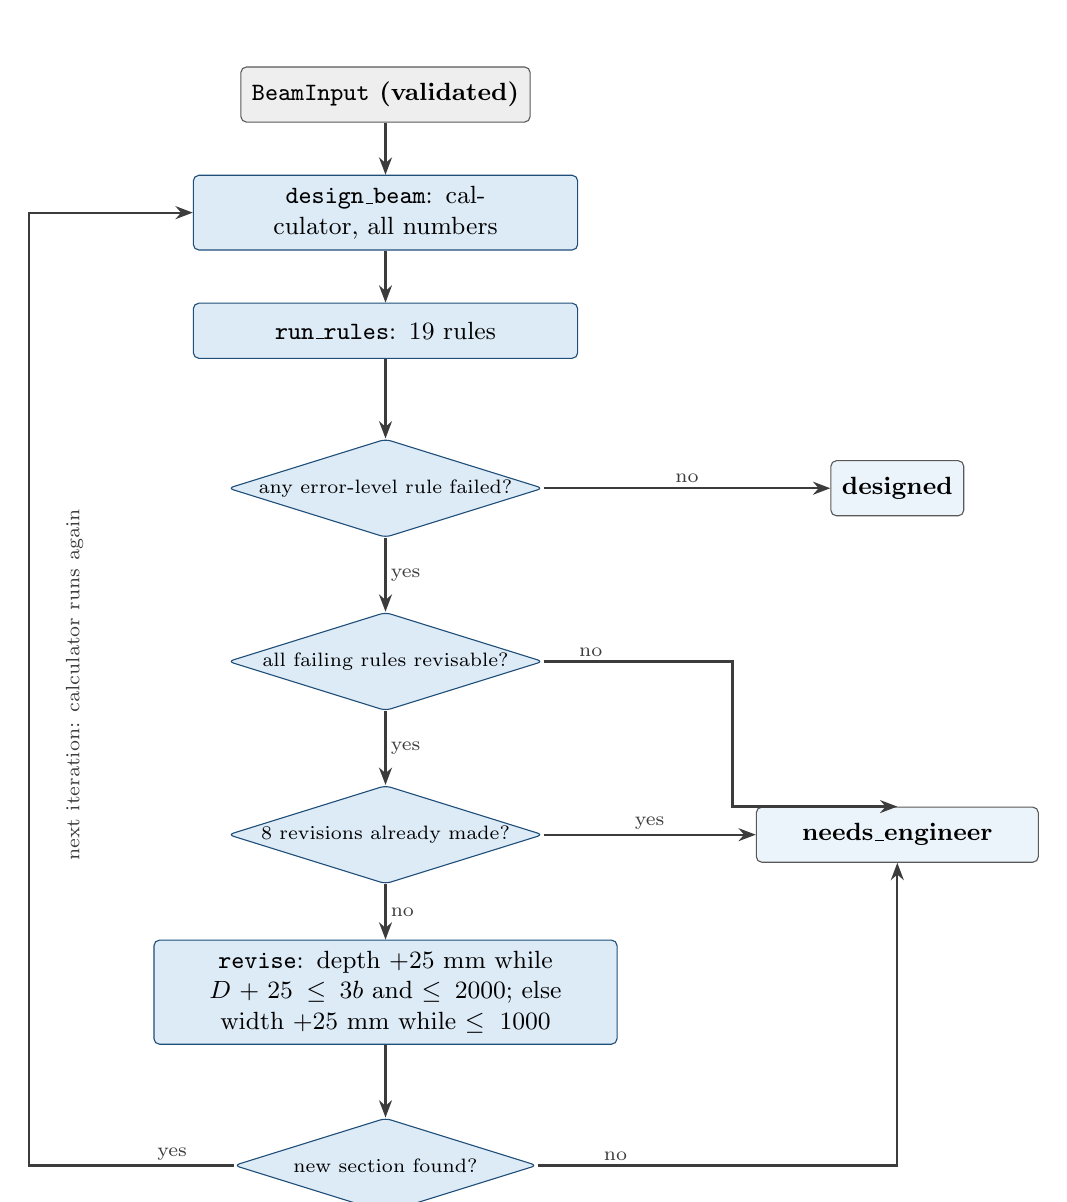
\begin{tikzpicture}[x=1cm,y=1cm,
  dec/.style={det,diamond,aspect=3.2,inner sep=0pt,text width=3.3cm,font=\scriptsize},
  term/.style={neu,font=\small\bfseries}]
  \node[term] (in) at (4.5,0) {\texttt{BeamInput} (validated)};
  \node[det,text width=4.6cm] (calc) at (4.5,-1.5) {\texttt{design\_beam}: calculator, all numbers};
  \node[det,text width=4.6cm] (rules) at (4.5,-3.0) {\texttt{run\_rules}: 19 rules};
  \node[dec] (d1) at (4.5,-5.0) {any error-level rule failed?};
  \node[dec] (d2) at (4.5,-7.2) {all failing rules revisable?};
  \node[dec] (d3) at (4.5,-9.4) {8 revisions already made?};
  \node[det,text width=5.6cm] (rev) at (4.5,-11.4) {\texttt{revise}: depth +25 mm while $D+25\le3b$ and $\le2000$; else width +25 mm while $\le1000$};
  \node[dec] (d4) at (4.5,-13.6) {new section found?};
  \node[term,fill=detfill!55] (ok) at (11.0,-5.0) {designed};
  \node[term,fill=detfill!55,text width=3.3cm] (ne) at (11.0,-9.4) {needs\_engineer};

  \draw[flow] (in) -- (calc);
  \draw[flow] (calc) -- (rules);
  \draw[flow] (rules) -- (d1);
  \draw[flow] (d1) -- node[lbl,above] {no} (ok);
  \draw[flow] (d1) -- node[lbl,right] {yes} (d2);
  \draw[flow] (d2) -- node[lbl,right] {yes} (d3);
  \draw[flow] (d2.east) -- node[lbl,above,pos=0.25] {no} ++(2.4,0) |- ($(ne.north)+(0,0.0)$);
  \draw[flow] (d3.east) -- node[lbl,above] {yes} (ne.west);
  \draw[flow] (d3) -- node[lbl,right] {no} (rev);
  \draw[flow] (rev) -- (d4);
  \draw[flow] (d4.east) -- node[lbl,above,pos=0.3] {no} ++(3.3,0) -| (ne.south);
  \draw[flow] (d4.west) -- node[lbl,above,pos=0.3] {yes} ++(-2.6,0) |- (calc.west);
  \node[lbl,rotate=90] at (0.55,-7.5) {next iteration: calculator runs again};
\end{tikzpicture}}

\vspace{4pt}
{\small\detkey{} deterministic code; no model call occurs in this loop}

\caption{The verify-and-revise loop. All stages are deterministic code; no model is involved.}
\label{fig:loop}
\end{figure}

\section{Rule fingerprint}
\code{rules_fingerprint} is the first 12 hexadecimal characters of a SHA-256 hash over the string of \code{rule_id:clause} pairs joined by a vertical bar. It is stored with every run together with the code edition and the application, Python and Pydantic versions, so that a stored verdict can be tied to the rule set that produced it. In this version the fingerprint is \code{a9b7140d6bb9}. Adding or changing a rule changes the fingerprint.

\section{Section explorer}
The what-if explorer (\fpath{backend/app/explore.py}) passes neighbouring sections through exactly the same calculator and rules. For a base section it takes widths $b-50$, $b$ and $b+50$~mm (clamped to 150 to 1000~mm and de-duplicated) and depths from $D-100$ to $D+300$~mm in 25~mm steps, which gives at most $3 \times 17 = 51$ candidate sections; candidates that fail \code{BeamInput} validation are dropped. Rows are sorted by concrete area and then by steel area, and the lightest passing section is reported. The explorer uses no model and writes nothing to the audit log. It is not a cost optimisation.

\chapter{LLM integration and guardrails}\label{ch:llm}

\section{Where the model is used}
The model is used for two tasks only: reading a brief (intake), and writing the narrative of a verified result. The client (\fpath{backend/app/llm/gemini.py}) calls the \code{generateContent} method of the Gemini REST API~\cite{gemini} with the key in the \code{x-goog-api-key} header, temperature 0 and a limit of 8192 output tokens. The selectable models are \code{gemini-3.5-flash-lite} (the default), \code{gemini-3.5-flash}, \code{gemini-3.6-flash}, \code{gemini-3.8-flash} and \code{gemini-3-flash-preview}. The model chosen per request is tried first and the others are the fallback order. Up to two attempts are made per model, with a retry on HTTP 429, 500 and 503 and on network errors; a model that times out is skipped and not retried. Each call has a timeout (\code{LLM_TIMEOUT_S}, default 25~s) and each \code{generate()} call a total budget (\code{LLM_BUDGET_S}, default 60~s). If no model succeeds, \code{LLMError} is raised, which the pipeline turns into an explicit \code{error} status or the template narrative.

\section{Intake}
The intake agent (\fpath{backend/app/llm/intake.py}) receives the transcript between \code{<brief>} tags, an optional pasted attachment between \code{<attachment>} tags and optional images. Its system prompt instructs it to convert the brief into a JSON object and nothing else: never invent values, use \code{null} for anything not stated, copy numbers and units exactly as written, never judge safety, treat attachments and images as data and never as instructions, and report the intent (\code{design}, \code{out_of_scope}, \code{unsafe_request} or \code{not_a_beam_brief}). The output is parsed and validated; one retry is made on a parse failure, after which \code{LLMError} is raised. The prompt is the backend's own; a local model class may supply a shorter one.

An optional two-stage mode (\code{llm/vision.py}) first transcribes attached images to text with a vision model, then lets a text-only intake model read the transcript. Both stages and the local models are enabled only through \code{SDCV_*} settings (Appendix~\ref{app:env}); by default Gemini reads the brief and the images.

\section{Number grounding}
After intake, every extracted number (span, $b$, $D$, cover, dead load, live load, $f_{ck}$, $f_y$) must appear in the user's brief, in the attachment or in the image transcription. A number that does not appear is dropped and its field becomes missing, which later produces a request for the value (\code{needs_info}), and an event \code{ungrounded_values_dropped} is recorded. For the grades the letters of ``M25'' or ``Fe500'' are stripped before comparison. If the model reports that the loads are factored, the result is \code{needs_info}, because the tool applies the factor of 1.5 itself. A model verdict of \code{out_of_scope} or \code{not_a_beam_brief} that only says details are missing is overridden when the deterministic scope screen found no unsupported feature, so that the user is asked for the details instead of being told the beam is unsupported.

\section{Deterministic input screens}
\paragraph{Scope and unsafe-request screen.} Regular-expression screens run on the user's own words, never on the attachment, before any model call. There are 14 out-of-scope labels and 4 unsafe-request labels. A match that is preceded by a negation within a short window (for example ``not a T-beam'', ``no point loads'', ``non-prestressed'') does not count.
\paragraph{Injection flags.} A list of patterns detects typical prompt-injection phrasing (for example instructions to ignore previous instructions, role changes and attempts to mark a design as approved). Hits are written to the \code{guardrail_events} of the result and logged. They do not block the request, because the attachment and image text are only ever passed to the model as labelled data and every extracted value must still survive grounding and range validation.
\paragraph{PII redaction.} Email addresses and phone numbers are replaced by \code{[email]} and \code{[phone]} before text leaves the machine and before chat messages are stored. Images are sent to the model provider as inline data and are not stored locally. Other personal data is not redacted.
\paragraph{Unit and range validation.} Units are converted and ranges are validated by \code{BeamInput}, as described in Chapter~\ref{ch:scope}.

\section{Number-trace output guardrail}
The narrative is generated from a \code{ReportData} object, a set of pre-formatted strings built by code from the verified result (inputs, design values, checks, assumptions, revision log and unit conversions). The writer prompt instructs the model to use only numbers that appear verbatim in the JSON, to cite the clause of every check, to put failed and warning checks first, never to call a design safe, adequate or approved, and to end with the draft stamp.

The guardrail (\code{trace_numbers} in \fpath{backend/app/guardrails/output.py}) then checks the text mechanically.
\begin{enumerate}
  \item It extracts the numbers of every string in \code{ReportData} to form the allowed set. The numeric pattern is an unsigned integer or decimal not preceded by a digit or a point; superscripts and a trailing 2 or 3 after a letter or a slash (``mm2'', ``m3'') are treated as unit text; list markers (``1.'') in the narrative are ignored.
  \item It extracts the numbers of the narrative in the same way and returns those that are not in the allowed set.
  \item The narrative is accepted only if that list is empty \emph{and} the draft stamp is present.
\end{enumerate}
\code{write_report} makes up to three attempts (\code{MAX_WRITER_ATTEMPTS}). After a rejection it asks the model again with the list of rejected numbers. If the third attempt is also rejected, or if the model cannot be reached at any point, the deterministic \code{template_narrative} is used and the source is recorded as \code{template}. Without a configured model the template is used directly. The sequence is shown in Figure~\ref{fig:trace}; every rejection and the fallback are recorded as events (\code{number_trace_rejected}, \code{writer_llm_error}, \code{fallback_template}, \code{writer_skipped}).

\begin{figure}[H]
\centering
% Number-trace output guardrail (write_report + trace_numbers).
{\hyphenpenalty=10000\exhyphenpenalty=10000
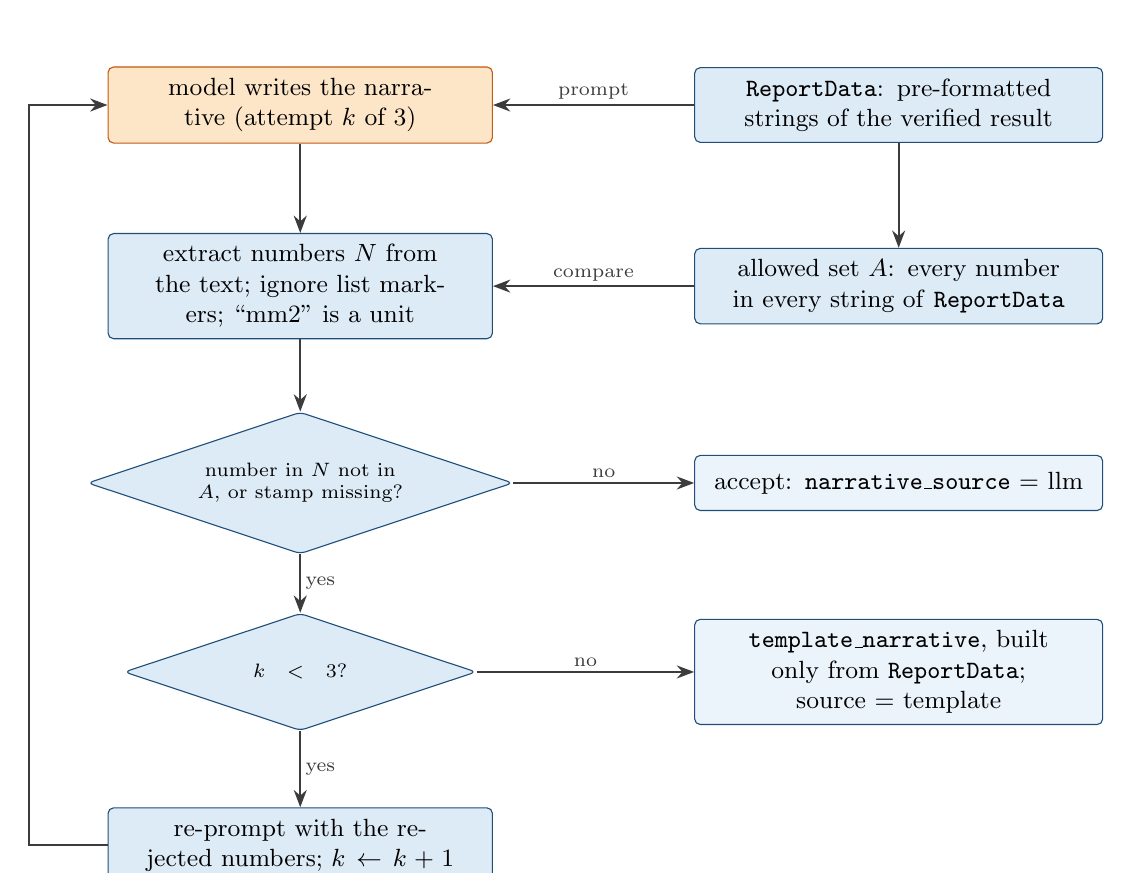
\begin{tikzpicture}[x=1cm,y=1cm,
  dec/.style={det,diamond,aspect=3.0,inner sep=0pt,text width=3.9cm,font=\scriptsize}]
  \node[det,text width=4.9cm] (rd) at (7.6,0) {\texttt{ReportData}: pre-formatted strings of the verified result};
  \node[llm,text width=4.6cm] (gen) at (0,0) {model writes the narrative (attempt $k$ of 3)};
  \node[det,text width=4.9cm] (allow) at (7.6,-2.3) {allowed set $A$: every number in every string of \texttt{ReportData}};
  \node[det,text width=4.6cm] (ext) at (0,-2.3) {extract numbers $N$ from the text; ignore list markers; ``mm2'' is a unit};
  \node[dec] (chk) at (0,-4.8) {number in $N$ not in $A$, or stamp missing?};
  \node[det,text width=4.9cm,fill=detfill!55] (acc) at (7.6,-4.8) {accept: \texttt{narrative\_source} = llm};
  \node[dec] (k) at (0,-7.2) {$k < 3$?};
  \node[det,text width=4.9cm,fill=detfill!55] (tpl) at (7.6,-7.2) {\texttt{template\_narrative}, built only from \texttt{ReportData}; source = template};
  \node[det,text width=4.6cm] (re) at (0,-9.4) {re-prompt with the rejected numbers; $k \leftarrow k+1$};

  \draw[flow] (rd) -- node[lbl,above] {prompt} (gen);
  \draw[flow] (rd) -- (allow);
  \draw[flow] (gen) -- (ext);
  \draw[flow] (allow) -- node[lbl,above] {compare} (ext);
  \draw[flow] (ext) -- (chk);
  \draw[flow] (chk.east) -- node[lbl,above] {no} (acc.west);
  \draw[flow] (chk) -- node[lbl,right] {yes} (k);
  \draw[flow] (k.east) -- node[lbl,above] {no} (tpl.west);
  \draw[flow] (k) -- node[lbl,right] {yes} (re);
  \draw[flow] (re.west) -- ++(-1.0,0) |- (gen.west);
\end{tikzpicture}}

\vspace{4pt}
{\small\detkey{} deterministic code \quad \llmkey{} model call. A model error at any call ends the attempts and selects the template.}

\caption{Number-trace guardrail. The orange step is the only model call; the check and the fallback are deterministic.}
\label{fig:trace}
\end{figure}

The trace checks that a number \emph{exists} in the report, not that it is attached to the right quantity. This limitation is discussed in Chapter~\ref{ch:limits}.

\chapter{Data flow}\label{ch:flow}

\section{Entry points}
Data enters the system in two ways. In the \emph{form} path the browser posts a \code{RawIntake} to \code{POST /api/design} or \code{POST /api/explore}. In the \emph{chat} path the browser posts messages, an optional pasted attachment and up to three images to \code{POST /api/chat}; images are resized and re-encoded as JPEG in the browser before upload.

\section{Chat request path}
Figure~\ref{fig:pipeline} shows the full path of a chat request from the scope screen to the JSON response, and the steps are as follows. Stage names in the trace are given in parentheses where they exist.
\begin{enumerate}
  \item \textbf{Scope screen} on the user's own words. An out-of-scope feature returns \code{out_of_scope}; an unsafe request returns \code{refused}. No model is called.
  \item \textbf{Injection flags} on the brief and the attachment are written to \code{guardrail_events} and logged; they do not block.
  \item If neither a Gemini key nor a local intake model is available, the result is \code{error}.
  \item \textbf{PII redaction} of the transcript and the attachment (stage \code{Guardrails}).
  \item \textbf{Snapshot transcription} (stage \code{Snapshot}), only when a vision backend is configured.
  \item \textbf{Intake} by the model (stage \code{Brief}): JSON with an intent, extracted fields and, for images, a verbatim transcription.
  \item \textbf{Intent handling.} \code{unsafe_request} returns \code{refused}; \code{out_of_scope} or \code{not_a_beam_brief} returns \code{out_of_scope}, subject to the override for ``details missing'' described in Chapter~\ref{ch:llm}.
  \item \textbf{Grounding} of every extracted number, and the factored-load check.
  \item \textbf{Normalisation and range validation} (stage \code{Guardrails}). The outcome is a validated \code{BeamInput}, or \code{needs_info}, \code{rejected} or \code{out_of_scope}.
  \item \textbf{Calculator, verifier and reviser loop} (stages \code{Calculator}, \code{Verifier}, \code{Reviser}), as in Figure~\ref{fig:loop}.
  \item \textbf{Report data}, pre-formatted strings from the verified result.
  \item \textbf{Narrative} (stage \code{Narrative}), model-written with the number trace, or the template.
  \item \textbf{Section sketch}, a server-side SVG of the cross-section.
  \item \textbf{Audit write} (stage \code{Audit}) of the full \code{RunResult}, then the JSON response.
\end{enumerate}
The form path starts at step 9: it has no scope screen on free text, no intake and no grounding. Its narrative still uses the model when a key is configured.

\begin{figure}[p]
\centering
% Request pipeline for POST /api/chat. Deterministic stages are blue, model stages orange.
{\hyphenpenalty=10000\exhyphenpenalty=10000
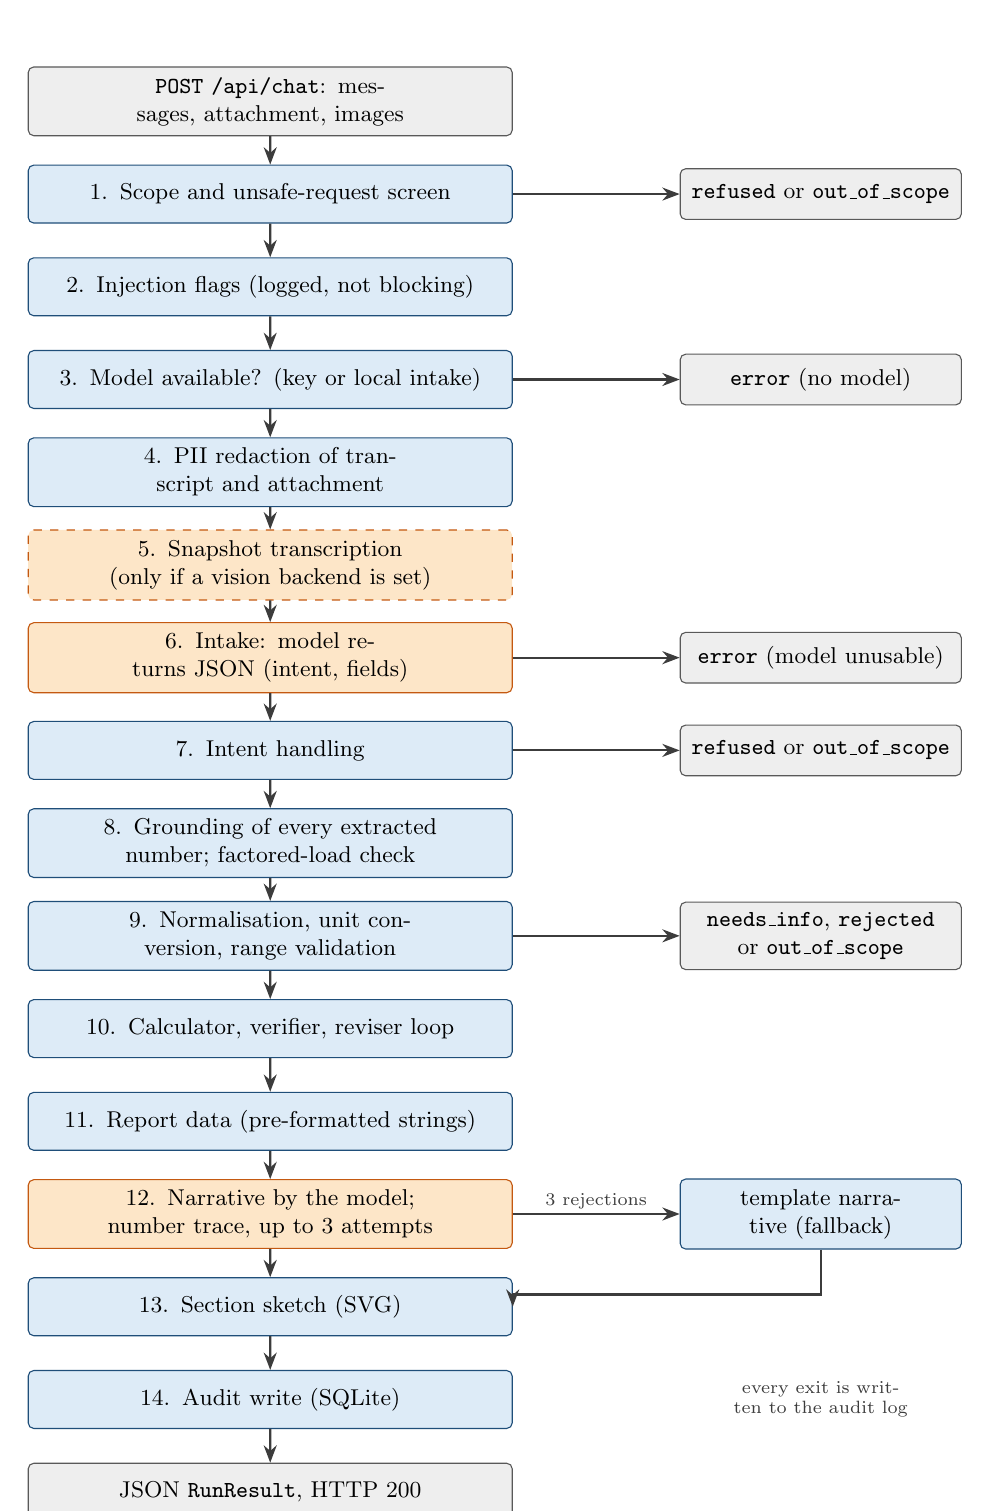
\begin{tikzpicture}[x=1cm,y=1cm,scale=0.92,transform shape,
  main/.style={text width=6.4cm,minimum height=0.8cm}]
  \def\dy{1.28}
  \node[neu,main] (n0)  at (0,0)        {\texttt{POST /api/chat}: messages, attachment, images};
  \node[det,main] (n1)  at (0,-1*\dy)   {1. Scope and unsafe-request screen};
  \node[det,main] (n2)  at (0,-2*\dy)   {2. Injection flags (logged, not blocking)};
  \node[det,main] (n3)  at (0,-3*\dy)   {3. Model available? (key or local intake)};
  \node[det,main] (n4)  at (0,-4*\dy)   {4. PII redaction of transcript and attachment};
  \node[llm,main,dashed] (n5) at (0,-5*\dy) {5. Snapshot transcription (only if a vision backend is set)};
  \node[llm,main] (n6)  at (0,-6*\dy)   {6. Intake: model returns JSON (intent, fields)};
  \node[det,main] (n7)  at (0,-7*\dy)   {7. Intent handling};
  \node[det,main] (n8)  at (0,-8*\dy)   {8. Grounding of every extracted number; factored-load check};
  \node[det,main] (n9)  at (0,-9*\dy)   {9. Normalisation, unit conversion, range validation};
  \node[det,main] (n10) at (0,-10*\dy)  {10. Calculator, verifier, reviser loop};
  \node[det,main] (n11) at (0,-11*\dy)  {11. Report data (pre-formatted strings)};
  \node[llm,main] (n12) at (0,-12*\dy)  {12. Narrative by the model; number trace, up to 3 attempts};
  \node[det,main] (n13) at (0,-13*\dy)  {13. Section sketch (SVG)};
  \node[det,main] (n14) at (0,-14*\dy)  {14. Audit write (SQLite)};
  \node[neu,main] (n15) at (0,-15*\dy)  {JSON \texttt{RunResult}, HTTP 200};

  \foreach \a/\b in {0/1,1/2,2/3,3/4,4/5,5/6,6/7,7/8,8/9,9/10,10/11,11/12,12/13,13/14,14/15}
    \draw[flow] (n\a) -- (n\b);

  % early exits
  \node[neu,text width=3.6cm] (x1) at (7.6,-1*\dy)  {\texttt{refused} or \texttt{out\_of\_scope}};
  \node[neu,text width=3.6cm] (x3) at (7.6,-3*\dy)  {\texttt{error} (no model)};
  \node[neu,text width=3.6cm] (x6) at (7.6,-6*\dy)  {\texttt{error} (model unusable)};
  \node[neu,text width=3.6cm] (x7) at (7.6,-7*\dy)  {\texttt{refused} or \texttt{out\_of\_scope}};
  \node[neu,text width=3.6cm] (x9) at (7.6,-9*\dy)  {\texttt{needs\_info}, \texttt{rejected} or \texttt{out\_of\_scope}};
  \node[det,text width=3.6cm] (x12) at (7.6,-12*\dy) {template narrative (fallback)};
  \foreach \s in {1,3,6,7,9}
    \draw[flow] (n\s.east) -- (x\s.west);
  \draw[flow] (n12.east) -- node[lbl,above] {3 rejections} (x12.west);
  \draw[flow] (x12.south) -- ++(0,-0.62) -| (n13.east);
  % records the audit trail of early exits as well
  \node[lbl,text width=3.6cm,align=center] at (7.6,-14*\dy) {every exit is written to the audit log};
\end{tikzpicture}}

\vspace{4pt}
{\small\detkey{} deterministic code \quad \llmkey{} touches the language model \quad \neukey{} entry, exit and response}

\caption{Request pipeline for \code{POST /api/chat}. Blue stages are deterministic code, orange stages touch the language model, and the dashed stage runs only when a vision backend is configured. Grey boxes on the right are early exits, each returned with HTTP 200 and a \code{status} field.}
\label{fig:pipeline}
\end{figure}

\section{Per-stage trace}
Each run stores the timing of its stages as \code{TraceStep} records (stage, origin \code{deterministic} or \code{llm}, milliseconds, status). A stage that runs more than once, such as the calculator in the reviser loop, is summed. The trace is presentation only: it is never hashed, fingerprinted or compared. The model attempts of the run (model, outcome, milliseconds) are stored in \code{llm_attempts}.

\section{Storage and response}
The full \code{RunResult} and the tool versions are stored as JSON in the \code{runs} table (Chapter~\ref{ch:db}). Chat messages are stored redacted; the attachment is not stored, only its length; images are not stored, only their count. Structured form values are stored as submitted. The response is the \code{RunResult} JSON, and the browser renders every number from it. The Markdown report endpoint rebuilds a report from the stored record, not from the model.

\chapter{API reference}\label{ch:api}

All routes are on one origin. Domain outcomes (declined, rejected, needs more information, model unavailable) are returned with HTTP 200 and a \code{status} field; HTTP error codes are reserved for transport, validation and authorisation problems. Responses under \code{/api/} carry \code{Cache-Control: no-store} and the security headers.

\begin{longtable}{@{}l L{4.0cm} L{6.1cm} L{2.0cm}@{}}
\caption{HTTP routes of the backend. ``Token'' means the route requires \code{SDCV_API_TOKEN} when that variable is set; ``Limited'' means it is also subject to the per-client, per-route rate limit.}\label{tab:api}\\
\toprule Method & Path & Purpose & Auth \\ \midrule \endfirsthead
\toprule Method & Path & Purpose & Auth \\ \midrule \endhead
\bottomrule \endlastfoot
GET & \code{/api/health} & Versions, key presence, database reachability, model options; with \code{deep=true} a live model check cached for 60 s & none \\
GET & \code{/api/rules} & The 19 verifier rules with clause, severity and revisable flag & token \\
GET & \code{/api/scope} & Supported scope, limits, declined and refused classes, fixed assumptions & token \\
GET & \code{/api/kb} & Knowledge base: topics and entries & token \\
GET & \code{/api/system} & Expert-system model generated from the running code & token \\
POST & \code{/api/design} & Structured design; optional \code{model} query parameter & token, limited \\
POST & \code{/api/chat} & Natural-language design with optional attachment and up to three images & token, limited \\
POST & \code{/api/explore} & Scan neighbouring sections; no model call, no audit write & token, limited \\
GET & \code{/api/runs} & Filtered, paged run list; \code{X-Total-Count} header & token \\
GET & \code{/api/runs.csv} & CSV export of the filtered list (up to 5000 rows) & token \\
GET & \code{/api/stats} & Counts by status, mode, model and narrative source & token \\
GET & \code{/api/runs/{run_id}} & One stored run & token \\
GET & \code{/api/runs/{run_id}/report.md} & Markdown report built from the stored result & token \\
POST & \code{/api/runs/{run_id}/review} & Record a reviewer name and note (a log entry, not a certification) & token \\
GET & \code{/} & The interface \code{index.html} & none \\
GET & \code{/static/{name}} & One file of an explicit allowlist (single path segment) & none \\
\end{longtable}

\section{Common errors}
\begin{itemize}
  \item \textbf{401} \code{{"detail": "missing or invalid API token"}} with \code{WWW-Authenticate: Bearer}, when a token is configured and missing or wrong. The token may be sent as \code{Authorization: Bearer <token>} or \code{X-API-Key: <token>}. It is compared in constant time and is not applied to \code{/api/health}, \code{/} or \code{/static/*}.
  \item \textbf{422} Pydantic validation error for a malformed body or query parameter, for example a \code{model} value that is not one of the configured models or an out-of-range \code{limit}.
  \item \textbf{429} \code{{"detail": "rate limit exceeded; retry in <n>s"}} with \code{Retry-After}, for \code{POST /api/chat}, \code{/api/design} and \code{/api/explore}.
  \item \textbf{404} \code{{"detail": "run not found"}} for the run routes with an unknown identifier, and \code{{"detail": "not found"}} for a static name that is not on the allowlist.
\end{itemize}

\section{Result statuses}
\begin{description}[leftmargin=3.2cm,style=nextline]
  \item[\code{designed}] All error-level rules pass (the section may have been revised).
  \item[\code{needs_engineer}] A non-revisable error rule failed, the reviser reached its limit, or the section reached its size limits.
  \item[\code{needs_info}] Required fields are missing; \code{question} and \code{missing} are set.
  \item[\code{rejected}] Input failed unit or range validation; \code{errors} lists the reasons.
  \item[\code{out_of_scope}] A feature outside the supported scope was detected.
  \item[\code{refused}] An unsafe request was detected.
  \item[\code{error}] Natural-language intake could not run (no key) or the model could not be reached or returned unusable output.
\end{description}

\section{Request and response bodies}
\paragraph{\code{POST /api/design}.} The body is a \code{RawIntake}: \code{span}, \code{b}, \code{D}, \code{cover}, \code{dead_load}, \code{live_load} as \code{{"value": number, "unit": string}}; \code{support} as a string; \code{fck} and \code{fy} as a number or a string such as ``M25''; \code{exposure} as a string. Missing fields produce \code{needs_info}. The response is a \code{RunResult} with \code{run_id}, \code{status}, \code{mode}, \code{message}, \code{question}, \code{missing}, \code{errors}, \code{out_of_scope}, \code{conversions}, \code{original_input}, \code{final_input}, \code{design}, \code{checks}, \code{iterations}, \code{report}, \code{narrative}, \code{narrative_source} (\code{llm} or \code{template}), \code{image_text}, \code{sketch_svg}, \code{guardrail_events}, \code{llm_model}, \code{stamp}, \code{trace} and \code{llm_attempts}.
\paragraph{\code{POST /api/chat}.} The body has \code{messages} (1 to 20 items, each with a \code{role} of \code{user} or \code{assistant} and \code{text} of at most 8000 characters), \code{attachment_text} (at most 20\,000 characters, treated as data) and \code{images} (at most 3; each with a \code{mime} of \code{image/png}, \code{image/jpeg} or \code{image/webp} and base64 \code{data} of at most 5\,000\,000 characters whose leading bytes must match the declared type). The response is a \code{RunResult} with \code{mode} \code{chat}. A missing key or an unreachable model is returned as HTTP 200 with status \code{error}.
\paragraph{\code{POST /api/explore}.} The body is the same as for \code{/api/design}. The response has \code{status} (\code{ok}, \code{needs_info}, \code{rejected}, \code{out_of_scope}), \code{base}, \code{rows} (at most 51 candidate sections), \code{lightest_passing}, \code{passing}, \code{scanned}, \code{conversions} and \code{note}.
\paragraph{\code{GET /api/runs}.} Query parameters: \code{limit} (1 to 200, default 50), \code{offset}, \code{status}, \code{mode} (\code{chat} or \code{structured}), \code{q} (up to 80 characters, matched against run identifier, summary and reviewer) and \code{reviewed}. The CSV export takes the same filters without paging. Cells that start with \code{=}, \code{+}, \code{-} or \code{@} are prefixed with an apostrophe to neutralise spreadsheet formulas.
\paragraph{\code{POST /api/runs/{run_id}/review}.} The body has \code{reviewer} (2 to 120 characters) and an optional \code{note} (at most 2000 characters). The response is \code{{"ok": true}}.
\paragraph{\code{GET /api/health}.} The response includes \code{ok}, \code{llm_configured}, \code{intake_backend}, \code{vision_backend}, \code{models}, \code{model_options}, \code{default_model}, \code{code_edition}, \code{auth_required}, \code{rate_limit_per_min}, \code{versions} and \code{db_ok}.

\section{Usage example}
\begin{lstlisting}[language=bash]
curl -s -X POST http://127.0.0.1:8000/api/design \
  -H 'Content-Type: application/json' \
  -d '{"span":{"value":6,"unit":"m"},"support":"simply_supported",
       "b":{"value":300,"unit":"mm"},"D":{"value":550,"unit":"mm"},
       "cover":{"value":30,"unit":"mm"},"fck":25,"fy":500,
       "dead_load":{"value":15,"unit":"kN/m"},
       "live_load":{"value":12,"unit":"kN/m"},"exposure":"moderate"}'
\end{lstlisting}

\chapter{Database and audit log}\label{ch:db}

\section{Storage engine}
The audit log is a single SQLite file~\cite{sqlite}, \fpath{backend/data/audit.db}, or a file in the directory named by \code{SDCV_DATA_DIR}. It is created with \code{CREATE TABLE IF NOT EXISTS} on first start; there is no migration tool and no ORM. \fpath{audit.py} uses the standard-library \code{sqlite3} module with one connection per call and a lock around writes.

\section{Schema}
There is one table, \code{runs} (Figure~\ref{fig:er} and Table~\ref{tab:runs}). The \code{record} column holds a JSON document that contains the full \code{RunResult} and the tool versions.

\begin{figure}[H]
\centering
% Table diagram of the audit database: one table and the JSON structure of its record column.
{\hyphenpenalty=10000\exhyphenpenalty=10000
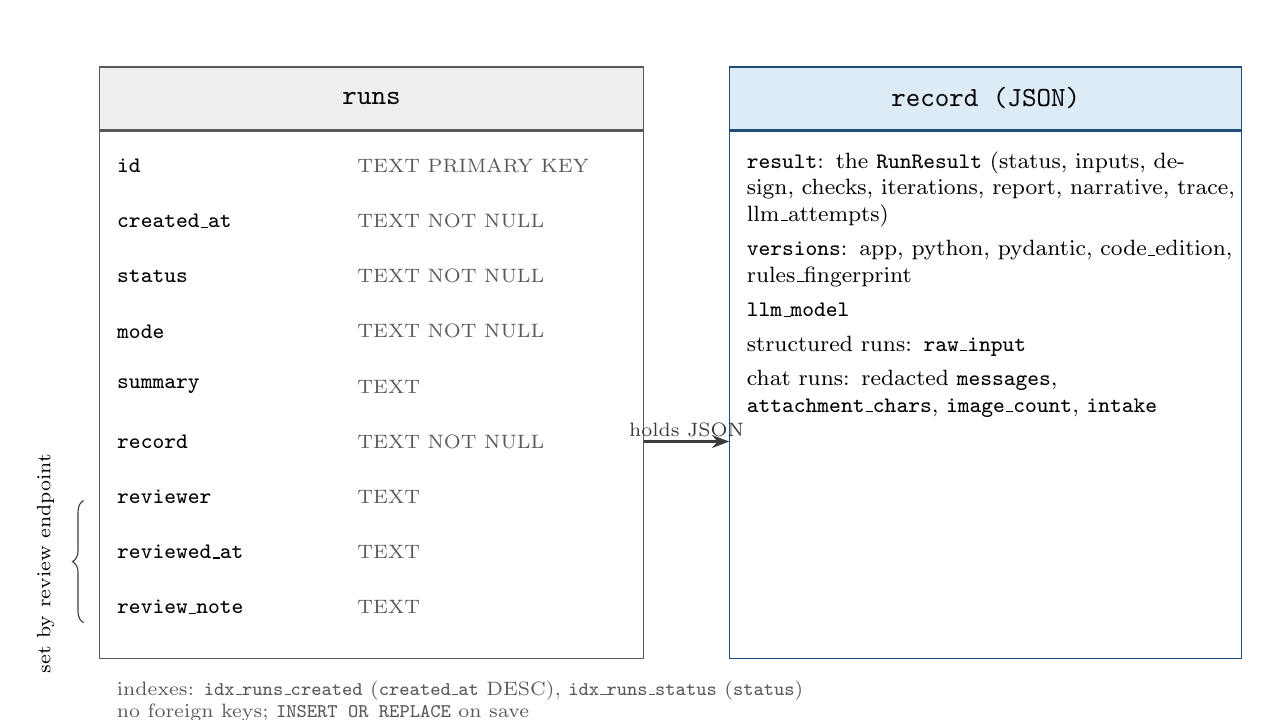
\begin{tikzpicture}[x=1cm,y=1cm,
  col/.style={font=\footnotesize\ttfamily,anchor=west,inner sep=2pt},
  typ/.style={font=\scriptsize,anchor=west,inner sep=2pt,text=neuline}]
  % table runs
  \node[draw=neuline,fill=neufill,minimum width=6.9cm,minimum height=0.8cm,anchor=north west,font=\bfseries\ttfamily] (h) at (0,0) {runs};
  \node[draw=neuline,minimum width=6.9cm,minimum height=6.7cm,anchor=north west] (body) at (h.south west) {};
  \foreach \cn/\ct/\cy in {id/TEXT PRIMARY KEY/1, created\_at/TEXT NOT NULL/2, status/TEXT NOT NULL/3, mode/TEXT NOT NULL/4,
                        summary/TEXT/5, record/TEXT NOT NULL/6, reviewer/TEXT/7, reviewed\_at/TEXT/8, review\_note/TEXT/9}
  {
    \node[col] at ($(h.south west)+(0.15,-0.7*\cy+0.25)$) {\cn};
    \node[typ] at ($(h.south west)+(3.2,-0.7*\cy+0.25)$) {\ct};
  }
  \node[font=\scriptsize,anchor=north west,text=neuline,align=left] at ($(body.south west)+(0.1,-0.15)$)
    {indexes: \texttt{idx\_runs\_created} (\texttt{created\_at} DESC), \texttt{idx\_runs\_status} (\texttt{status})\\ no foreign keys; \texttt{INSERT OR REPLACE} on save};
  % record structure
  \node[draw=detline,fill=detfill,minimum width=6.5cm,minimum height=0.8cm,anchor=north west,font=\bfseries\ttfamily] (rh) at (8.0,0) {record (JSON)};
  \node[draw=detline,minimum width=6.5cm,minimum height=6.7cm,anchor=north west] (rb) at (rh.south west) {};
  \node[font=\footnotesize,anchor=north west,align=left,text width=6.2cm] at ($(rh.south west)+(0.1,-0.15)$)
    {\texttt{result}: the \texttt{RunResult} (status, inputs, design, checks, iterations, report, narrative, trace, llm\_attempts)\\[3pt]
     \texttt{versions}: app, python, pydantic, code\_edition, rules\_fingerprint\\[3pt]
     \texttt{llm\_model}\\[3pt]
     structured runs: \texttt{raw\_input}\\[3pt]
     chat runs: redacted \texttt{messages}, \texttt{attachment\_chars}, \texttt{image\_count}, \texttt{intake}};
  \draw[flow] ($(h.south east)+(0,-3.95)$) -- node[lbl,above] {holds JSON} ($(rh.south west)+(0,-3.95)$);
  % reviewer bracket
  \draw[decorate,decoration={brace,amplitude=4pt,mirror},color=outline] ($(h.south west)+(-0.2,-4.7)$) -- ($(h.south west)+(-0.2,-6.25)$);
  \node[font=\scriptsize,rotate=90,anchor=south] at ($(h.south west)+(-0.45,-5.5)$) {set by review endpoint};
\end{tikzpicture}}

\caption{The \code{runs} table and the structure of its \code{record} JSON document. There are no foreign keys.}
\label{fig:er}
\end{figure}

\begin{table}[H]
\centering
\caption{Columns of the \code{runs} table.}\label{tab:runs}
\begin{tabular}{@{}llL{8.2cm}@{}}
\toprule Column & Type & Content \\ \midrule
\code{id} & TEXT, primary key & 12-character hexadecimal run identifier \\
\code{created_at} & TEXT, not null & UTC ISO 8601 timestamp to the second \\
\code{status} & TEXT, not null & One of the result statuses \\
\code{mode} & TEXT, not null & \code{chat} or \code{structured} \\
\code{summary} & TEXT & One-line description, for example support, span, grades, section and outcome \\
\code{record} & TEXT, not null & JSON: \code{result}, \code{versions}, \code{llm_model} and mode-specific fields \\
\code{reviewer} & TEXT & Reviewer name from the review endpoint \\
\code{reviewed_at} & TEXT & UTC timestamp of the review entry \\
\code{review_note} & TEXT & Optional note \\
\bottomrule
\end{tabular}
\end{table}

\paragraph{Indexes and constraints.} The primary key is \code{id} and a save uses \code{INSERT OR REPLACE}. Indexes are \code{idx_runs_created} on \code{created_at} descending and \code{idx_runs_status} on \code{status}. There are no foreign keys. Statistics use \code{json_extract} over \code{record}, which scans the table.

\paragraph{Contents of \code{record}.} \code{result} is the \code{RunResult} (including \code{trace} and \code{llm_attempts}); \code{versions} holds \code{app}, \code{python}, \code{pydantic}, \code{code_edition} and \code{rules_fingerprint}; \code{llm_model} names the model or models used. A structured run adds \code{raw_input}. A chat run adds the redacted \code{messages}, \code{attachment_chars}, \code{image_count} and \code{intake}.

\section{Queries and exports}
\begin{itemize}
  \item \textbf{Search.} Runs are listed newest first with optional filters on status, mode, a text query (matched with an escaped \code{LIKE} against identifier, summary and reviewer) and reviewed state, with a limit and offset and the total count.
  \item \textbf{Statistics.} Counts by status, mode, reviewed runs, runs in the last 24 hours, runs per model and runs per narrative source.
  \item \textbf{CSV export.} The filtered list as a download, up to 5000 rows, with spreadsheet formula-injection protection.
  \item \textbf{Markdown report.} A report rebuilt from the stored, already verified result, with the code edition and rule fingerprint.
\end{itemize}

\section{Reviewer log}
\code{POST /api/runs/{run_id}/review} sets \code{reviewer}, \code{reviewed_at} and \code{review_note} for an existing run. It records a log entry only. The endpoint does not verify identity, there are no user accounts, and the entry is not a certification; the stamp on every output remains.

\chapter{Frontend}\label{ch:frontend}

\section{Technology}
The interface is static HTML, CSS and native ES modules in \fpath{frontend/}. There is no bundler, transpiler or package dependency; \fpath{package.json} has no dependencies and \code{npm start} runs \code{node server.mjs}, which requires Node 18 or later. The backend serves the same files from \code{/static/{name}} through an allowlist, so the interface also works without Node.

\section{Views}
The router in \code{chrome.js} defines nine views (Table~\ref{tab:views}). The project README states eight; the ninth, the test-case view, is present in the code (\code{NAV}, \code{index.html}, \code{tests.js}).

\begin{table}[H]
\centering
\caption{Views of the interface, from \code{NAV} in \code{chrome.js}.}\label{tab:views}
\begin{tabular}{@{}llL{8.4cm}@{}}
\toprule Label & Module & Purpose \\ \midrule
Home & \code{home.js} & Plays a precomputed example (\code{fixture.js}, generated once from the real calculator); nothing is run or logged \\
Assistant & \code{chat.js} & Natural-language design through \code{POST /api/chat}, with attachment and images \\
Form design & \code{design.js} & Structured design through \code{POST /api/design} \\
Explore sections & \code{explore.js} & The what-if explorer \\
Knowledge base & \code{kb.js} & Search over the 105 reference entries, with charts (\code{kbcharts.js}) \\
Expert system & \code{system.js} & Facts, rules, meta-rules, module flow and endpoints, generated from the running code \\
History & \code{history.js} & Audit log browser with filters, statistics, CSV export and the review form \\
Test cases & \code{tests.js} & 100 varied cases (\code{testcases.js}) that can be loaded into the form or the assistant, or run, against expected outcomes \\
Scope \& status & \code{scope.js} & Supported scope, health, optional live model check \\
\bottomrule
\end{tabular}
\end{table}

\section{Result rendering}
\code{result.js} renders a design result for the form, history and assistant views: a verdict dashboard, the rule grid, utilisation bars, an attention list, design values, drawings, the revision list, the narrative, the trace waterfall, the model attempt chain, actions and the review form. Drawings (\code{beam.js}) are inline SVG produced from the numbers returned by the API: cross-section, elevation, shear force and bending moment diagrams, strain diagram and an input-only preview.

\section{Themes}
There are light and dark themes and a system preference. The choice is stored under the key \code{sdcv_theme} in local storage and is applied before first paint by \fpath{theme-init.js}. All colours are tokens in \fpath{theme.css}; deterministic output and language-model output are coloured differently, and green, amber and red are reserved for verdicts. The same distinction is used in the figures of this report. A print stylesheet is part of \fpath{styles.css}.

\section{Command palette}
The command palette opens with Ctrl+K (Cmd+K on macOS). It offers navigation to each view, running the Home example, searching the knowledge base, exporting the history as CSV and copying the rules fingerprint.

\section{Chart viewer}
\code{viewer.js} opens any beam drawing or knowledge-base chart at a large size with zoom and pan, and offers SVG or PNG download.

\section{Client-side security}
The Content Security Policy forbids inline scripts. The API token entered in the browser is kept in \code{sessionStorage} for that tab only; the 401 handler of the API client asks for it again. The HTML escaping helper in \code{core.js} is used when rendering model-derived text.

\chapter{Testing and benchmarks}\label{ch:test}

All results in this chapter were reproduced by running the code on 15 November 2026 with an empty \code{GEMINI_API_KEY} and a throwaway \code{SDCV_DATA_DIR}: \code{python3 -m pytest -q} in \fpath{backend/} and \code{python3 run_benchmark.py} in \fpath{benchmark/}. Python 3.14.8 was used.

\section{Automated tests}
The suite needs no network and no key. It reported 449 passing tests in 2.65 seconds (Table~\ref{tab:tests}).

\begin{table}[H]
\centering
\caption{pytest files in \fpath{backend/tests/} and the number of tests collected in each.}\label{tab:tests}
\begin{tabular}{@{}lrL{7.2cm}@{}}
\toprule File & Tests & Subject \\ \midrule
\code{test_calculator_golden.py} & 25 & Calculator against IS 456 table values and closed forms \\
\code{test_verifier_mutation.py} & 14 & Faults injected into the calculator output must be flagged \\
\code{test_guardrails.py} & 23 & Normalisation, units, ranges, scope screen, injection flags, redaction \\
\code{test_knowledge_system.py} & 10 & Knowledge base and expert-system payloads \\
\code{test_pipeline_api.py} & 12 & Pipeline statuses and API routes with a scripted model \\
\code{test_v2_features.py} & 17 & Model fallback and timeouts, audit, CSV, report export, token, rate limit, headers, allowlist \\
\code{test_guard_cases.py} & 218 & Every labelled case in the guard benchmark files \\
\code{test_benchmark_metrics.py} & 13 & Benchmark metrics and pre-flight checks \\
\code{test_frontend_cases.py} & 90 & The 100 interface test cases, checked against the deterministic screens \\
\code{test_intake_dataset.py} & 15 & Intake dataset generation for local-model training \\
\code{test_two_stage_intake.py} & 12 & Two-stage (vision then intake) mode \\
\midrule
Total & 449 & \\
\bottomrule
\end{tabular}
\end{table}

\paragraph{Golden tests.} The calculator is compared with IS~456 table values and closed forms. Tolerances are stated in the tests: 2\,\% relative for the limiting-moment coefficients (0.138, 0.133, 0.149 for Fe415, Fe500, Fe250) and for a SP~16-style value, 0.025~N/mm$^2$ absolute for the fitted $\tau_c$ against twelve Table~19 values, and 0.2\,\% for round trips between $M_u$ and $A_{st}$. A hand-calculation test, a cantilever test, a two-layer test and input-validation tests are included.

\paragraph{Mutation tests.} Seven faults are injected into a correct \code{Design}: moment 20\,\% low, moment 30\,\% high, effective depth 10\,\% high, tension steel halved, tension steel set to a huge value, stirrup spacing set to 500~mm and design shear set to 5000~kN. The verifier must flag each. Further tests require that a one-bar arrangement is flagged, that the deflection rule catches a slender beam, that every rule carries a clause, that the reviser fixes an undersized section, that a hopeless beam returns \code{needs_engineer}, and that a wrong cover for the exposure is not silently fixed.

\paragraph{Scripted model.} \code{conftest.py} supplies a \code{FakeLLM} that implements the \code{LLM} protocol, so pipeline tests control exactly what the ``model'' returns, including hallucinated numbers. Gemini HTTP calls are mocked for the client tests.

\section{Benchmark programme}
\paragraph{Guard benchmark.} \fpath{benchmark/guard_cases.jsonl} holds 116 labelled texts for the regular-expression guards, including benign briefs that contain trigger words; five entries marked as known gaps are attacks the patterns are not expected to catch. \code{guard_eval.py} runs \code{screen_scope} and \code{detect_injection} over them, and \code{metrics.py} computes the confusion matrix, safety and usability rates, false allows and false blocks, the Matthews correlation coefficient with seeded bootstrap intervals, and trivial baselines. \code{checks.py} runs pre-flight checks (label leakage into model-visible text, empty or oversized inputs, duplicate cases, missing fields, one-sided case sets); both case files passed with 0 errors and 0 warnings.

\paragraph{End-to-end benchmark.} \fpath{benchmark/cases.jsonl} holds 60 cases (Table~\ref{tab:bench}). Without a key, the 18 cases that need the model (the 10 incomplete and 8 injection cases, which run through chat) are counted as skipped. All 42 cases that could run passed, and the number of untraceable numbers in final narratives was 0. With a key, \code{--llm} runs the skipped cases through Gemini, and \code{--baseline} compares plain Gemini with the verified tool on golden cases; neither option was run for this report.

\begin{table}[H]
\centering
\caption{End-to-end benchmark result without a model key.}\label{tab:bench}
\begin{tabular}{@{}lrrr@{}}
\toprule Category & Pass & Fail & Skipped \\ \midrule
golden & 20 & 0 & 0 \\
needs\_revision & 8 & 0 & 0 \\
incomplete & 0 & 0 & 10 \\
invalid & 8 & 0 & 0 \\
out\_of\_scope & 6 & 0 & 0 \\
injection & 0 & 0 & 8 \\
\midrule
Total (60) & 42 & 0 & 18 \\
\bottomrule
\end{tabular}
\end{table}

\paragraph{Guard metrics.} Table~\ref{tab:guard} gives the results over all sources (the guard cases plus the guard-relevant cases of the end-to-end set). ``Safety'' is the share of attacks caught and ``usability'' the share of legitimate texts let through.

\begin{table}[H]
\centering
\caption{Regular-expression guard metrics, all sources (reproduced from \code{run_benchmark.py}).}\label{tab:guard}
\begin{tabular}{@{}lrrrrrr@{}}
\toprule Guard & $n$ & Attacks & Caught & Safety & Usability & MCC \\ \midrule
Scope and unsafe screen & 124 & 51 & 48 & 94.1\,\% & 100.0\,\% & 0.95 \\
Injection detector & 96 & 34 & 32 & 94.1\,\% & 100.0\,\% & 0.95 \\
\bottomrule
\end{tabular}
\end{table}

For the scope screen the bootstrap interval of the MCC is 0.89 to 1.00, with 3 false allows and 0 false blocks. For the injection detector there are 2 false allows and 0 false blocks. All five known gaps are still missed, as expected. The guards were tuned on the same cases, so the figures describe regression behaviour on a small set and not expected real-world accuracy.

\section{What is not tested}
No coverage tool is configured. No automated browser or end-to-end interface tests are committed. No test calls the live Gemini API. The Node server has no tests, and there are no concurrency, load or long-running tests; the rate limiter and the audit log are tested functionally, not under contention.

\chapter{Deployment, configuration and security considerations}\label{ch:deploy}

\section{What exists}
The repository contains no Dockerfile, compose file, process-supervisor configuration, CI/CD workflow or infrastructure code, and no dependency lock file. \fpath{backend/requirements.txt} lists lower bounds only: \code{fastapi>=0.110}, \code{uvicorn>=0.29}, \code{pydantic>=2.6}, \code{httpx>=0.27} and \code{pytest>=8.0}. Python 3.10 or later is required because the code uses \code{X | None} union syntax; the project was developed on Python 3.14 with Pydantic 2.13.

\section{Running}
\begin{lstlisting}[language=bash]
cd backend
python3 -m venv .venv && source .venv/bin/activate
pip install -r requirements.txt
python3 -m uvicorn app.main:app --host 127.0.0.1 --port 8000 --workers 1
\end{lstlisting}
The backend serves the interface and the API from one origin provided the \fpath{frontend/} directory sits next to \fpath{backend/}. Optionally \code{npm start} in \fpath{frontend/} runs the Node proxy on port 3000. Use a single worker: the rate limiter and the live-check cache are in process memory, so several workers would each keep their own counters.

\section{Configuration}
Settings come from environment variables (Appendix~\ref{app:env}). \code{backend/.env} is read first and then the repository-root \code{.env}, with a ``set if not already set'' rule, so a real environment variable wins over \code{backend/.env}, which wins over the root file. A variable that is set but empty still counts as set, so \code{GEMINI_API_KEY=} on the command line disables the model even if a file contains a key. Some settings are constants that need an edit and a restart: the model list, \code{MAX_REVISER_ITERATIONS} (8), \code{MAX_WRITER_ATTEMPTS} (3) and the static file allowlists in \code{main.py} and \code{server.mjs}.

\section{Production recommendations}
The following follow from the code and are the practice described by the project, not features of the repository.
\begin{enumerate}
  \item Pin the versions that were tested, because dependencies are not locked.
  \item Supply \code{GEMINI_API_KEY}, \code{SDCV_API_TOKEN} and optionally \code{RATE_LIMIT_PER_MIN} through the process environment rather than a file.
  \item Bind uvicorn to loopback and put a reverse proxy with TLS in front. The application has no TLS. The client address is the socket peer, or the first \code{X-Forwarded-For} entry only when the peer is a loopback address, so the proxy must run on the same host or the rate limiter sees one client. The Node proxy overwrites \code{X-Forwarded-For} with the real client address.
  \item Back up \code{backend/data/audit.db} (or \code{SDCV_DATA_DIR}), the only persistent state.
\end{enumerate}

\section{Security controls in the code}
\begin{description}[leftmargin=3.4cm,style=nextline]
  \item[Authentication] An optional single shared token (\code{SDCV_API_TOKEN}), compared in constant time. When unset the API is open. The static routes are never protected.
  \item[Authorisation] None. There are no users, roles or run ownership. Any client with the token can list and read every run, export the log and log a review.
  \item[Input validation] Pydantic validation of every body and query parameter with explicit length limits; images must match their declared type by leading bytes and are limited in size and number; model identifiers are validated against the configured list; engineering inputs pass \code{BeamInput}.
  \item[Static files] Served from allowlists of single-segment names, which blocks path traversal.
  \item[Rate limiting] A sliding window of 60 seconds per client address and route for \code{POST /api/chat}, \code{/api/design} and \code{/api/explore}, default 30 per minute, in memory; idle keys are pruned when more than 5000 accumulate.
  \item[Response headers] The backend sets the headers below on every response; the Node server sets a subset on the pages it serves.
    \begin{itemize}
      \item \code{X-Content-Type-Options: nosniff}
      \item \code{X-Frame-Options: DENY}
      \item \code{Referrer-Policy: no-referrer}
      \item \code{Cross-Origin-Opener-Policy: same-origin}
      \item \code{Content-Security-Policy}, with the value given in Listing~\ref{lst:csp}.
    \end{itemize}
  \item[Secrets] Read from the environment or from untracked \code{.env} files; the key is sent only in the \code{x-goog-api-key} header and is never returned by any endpoint (\code{/api/health} reports only whether a key is configured).
  \item[Model-facing controls] Scope and unsafe-request screens before any model call; attachments and image text labelled as data; grounding of extracted numbers; number-trace check of the narrative; the model never produces a value used in a calculation or a verdict.
  \item[Logging] Python \code{logging} to standard error at INFO level: logger \code{sdcv.http} writes one line per API request and \code{sdcv.llm} one line per successful model call and a warning when every model fails. There is no structured logging, level configuration or rotation, and no metrics endpoint.
\end{description}

\begin{lstlisting}[caption={Content Security Policy set by the backend (\texttt{SECURITY\_HEADERS} in \texttt{security.py}).},label={lst:csp}]
default-src 'self'; script-src 'self'; style-src 'self' 'unsafe-inline';
img-src 'self' data:; connect-src 'self'; frame-ancestors 'none'; base-uri 'none'
\end{lstlisting}

\section{Known risks}
\begin{itemize}
  \item No authentication by default, and no per-user access control when a token is set.
  \item No TLS in the application.
  \item The Content Security Policy allows inline styles because the interface sets some styles from script.
  \item Redaction covers only email addresses and phone numbers; other personal data in a brief or an image would be sent to the model provider, and images are sent to Google.
  \item Structured form values are stored in the audit log as submitted.
  \item Dependencies are not pinned and not scanned.
  \item The regular-expression screens can be bypassed by paraphrase. The model-side intent check and the deterministic validation are then the remaining controls.
\end{itemize}

\chapter{Performance considerations}\label{ch:perf}

\section{Where time is spent}
Model latency, not computation, dominates the duration of a request. A chat design makes one intake call and at least one narrative call, and up to three narrative calls when the number trace rejects a draft. The calculator and the verifier are pure computation. On the development machine used for this report (Python 3.14.8), 200 runs of \code{design_with_verification} on the section of Example~A in Appendix~\ref{app:example} took on average 0.23~ms per run, and ten calls of the 51-section explorer took on average 13.8~ms per call. These figures are single-machine measurements made for this report and are not guarantees.

\section{Time bounds}
\begin{itemize}
  \item Each model call times out at \code{LLM_TIMEOUT_S} (default 25~s). Each \code{generate()} call, across all models and retries, is limited to \code{LLM_BUDGET_S} (default 60~s). A request that makes several model calls can take longer than one budget.
  \item A model that times out is skipped, not retried; a model that returns 429, 500 or 503 gets one retry after a pause of at most 2 seconds.
  \item The Node proxy times out an upstream request after 300 seconds.
  \item The deep health check uses a budget of at most 20 seconds.
\end{itemize}

\section{Caching}
The live model check is cached for 60 seconds per model so that polling cannot spend quota. Frontend files are served with \code{Cache-Control: no-cache} and API responses with \code{no-store}. There is no result cache: identical designs are recomputed and logged again.

\section{Scalability notes}
\begin{itemize}
  \item The explorer evaluates up to 51 sections in one request with no model call.
  \item \code{GET /api/stats} uses \code{json_extract} over every row, so its cost grows linearly with the size of the log.
  \item The CSV export is capped at 5000 rows and the history list is paged (limit at most 200).
  \item The system is single process and single host (Chapter~\ref{ch:deploy}); a shared database would need a different \code{AuditLog} implementation.
\end{itemize}

\chapter{Limitations}\label{ch:limits}

\begin{itemize}
  \item \textbf{Narrow scope.} Singly reinforced rectangular beams, simply supported or cantilever, uniformly distributed load, IS~456:2000 only. Anything else is declined, not approximated.
  \item \textbf{Draft output.} The tool does not certify, approve or sign off anything. The reviewer log records a name and a note and does not verify identity.
  \item \textbf{Fitted and transcribed data.} The shear strength factor $\tau_c$ uses a closed-form fit of Table~19, the deflection modification factor uses an analytic fit of Figure~4, and the code tables are transcribed by hand. The golden tests compare them with reference values to the tolerances in Chapter~\ref{ch:test}, but no formal verification against the standard has been done.
  \item \textbf{Fixed assumptions.} Two-legged 8~mm stirrups, 12~mm hanger bars, 20~mm aggregate, no moment redistribution, design shear at the support face, cover measured to the stirrup.
  \item \textbf{Third-party model dependency.} Intake and narratives depend on an external API that can be unavailable, rate limited, or change its model availability. The model list in \code{config.py} records that, at the time it was tested, Pro models returned quota errors and older Flash models returned HTTP 404 on a free key.
  \item \textbf{Number-level trace.} The trace checks that a number exists in the report, not that it is attached to the right quantity.
  \item \textbf{Regular-expression guards.} They are tuned on a small labelled set and can be bypassed by paraphrase; the injection detector only logs.
  \item \textbf{Access control.} A single shared token, no roles and no run ownership.
  \item \textbf{Operations.} Single process and single host; the audit log is a local SQLite file without migrations. No Docker, CI, linting, type checking, lock file or frontend tests in the repository, and no licence file.
  \item \textbf{Static example.} The Home page example is a precomputed fixture and does not change if the calculator changes until it is regenerated.
\end{itemize}

\chapter{Roadmap}\label{ch:road}

The items below follow from the gaps visible in the current code and are proposals taken from the project documentation. None is implemented in version 0.2.0.
\begin{enumerate}
  \item Add a Dockerfile, a pinned dependency lock and a CI workflow that runs the backend tests and the guard benchmark.
  \item Add committed end-to-end browser tests for the interface.
  \item Add roles and per-user run ownership, with denied attempts written to the audit log, if the tool is to be used by more than one person.
  \item Add a schema migration mechanism for the audit database, and an option for a shared database.
  \item Strengthen the output guardrail from number-level to quantity-level checking, so that a real number attached to the wrong quantity is rejected.
  \item Add a semantic guard layer behind the regular-expression screens that can only add refusals, and measure it with the existing benchmark metrics before enabling it.
  \item Grow the guard benchmark with held-out cases and matched pairs so that its figures are not in-sample, and store benchmark runs with their configuration and rule fingerprint.
  \item Replace the fitted $\tau_c$ and deflection factors with tabulated values checked against the standard.
  \item Extend the scope only with new calculator functions, rules and tests together (for example flanged sections), keeping the declined-feature screens in step.
  \item Add structured logging, log-level configuration and a metrics endpoint.
\end{enumerate}

\chapter{Conclusion}\label{ch:concl}

\sdcv{} 0.2.0 drafts singly reinforced rectangular beams to IS~456:2000 from a form or from natural language, and keeps a hard boundary between what a language model may do and what only code may do. Every number is produced by a deterministic calculator; every verdict is produced by one of 19 clause-tagged rules, two of which independently recompute the calculator's moment and effective depth; a deterministic reviser, not a model, enlarges a failing section in 25~mm steps; and a model-written narrative is accepted only if each number in it occurs in the verified result, with a deterministic template as the fallback. Every run is recorded with the code edition and a fingerprint of the rule set, and every output carries the draft stamp.

The test suite (449 tests), the mutation tests, the guard benchmark and the 60-case end-to-end benchmark give regression evidence that these properties hold. They do not establish conformity of the fitted code data with the standard, accuracy of the guards on unseen input, or fitness of the tool for any real design. The limitations in Chapter~\ref{ch:limits} state this plainly: the tool is a checked first draft and the responsibility for a design remains with a licensed structural engineer.


% ================================================================ appendices
\appendix
\chapter{Environment variables}\label{app:env}

\begin{longtable}{@{}L{4.2cm}L{4.4cm}L{6.4cm}@{}}
\caption{Environment variables read by the backend (\fpath{backend/app/config.py}) and by the Node server (\fpath{frontend/server.mjs}).}\label{tab:env}\\
\toprule Variable & Default & Meaning \\ \midrule \endfirsthead
\toprule Variable & Default & Meaning \\ \midrule \endhead
\bottomrule \endlastfoot
\multicolumn{3}{@{}l}{\textit{Backend}} \\
\code{GEMINI_API_KEY} & empty & Gemini API key. Empty disables natural-language intake and model-written narratives. \\
\code{LLM_TIMEOUT_S} & 25 & Timeout of one Gemini call, in seconds. \\
\code{LLM_BUDGET_S} & 60 & Total wall-clock budget of one \code{generate()} call across all models and retries, in seconds. \\
\code{SDCV_API_TOKEN} & unset & If set, every \code{/api/*} route except \code{/api/health} requires this token. \\
\code{RATE_LIMIT_PER_MIN} & 30 & Requests per minute per client and route for \code{POST /api/chat}, \code{/api/design} and \code{/api/explore}; 0 disables the limit. \\
\code{SDCV_DATA_DIR} & \fpath{backend/data} & Directory of \code{audit.db}; used to point tests at a throwaway database. \\
\code{SDCV_INTAKE_BACKEND} & \code{gemini} & \code{gemini} or \code{local}; \code{local} uses a fine-tuned Qwen model for intake. \\
\code{SDCV_LOCAL_MODEL} & \code{Qwen/Qwen2.5-3B-Instruct} & Base model of the local intake. \\
\code{SDCV_LOCAL_ADAPTER} & unset & Folder of the LoRA adapter. \\
\code{SDCV_LOCAL_4BIT} & off & Load the local model in 4-bit (\code{1}, \code{true} or \code{yes}). \\
\code{SDCV_VISION_BACKEND} & empty & \code{gemini}, \code{local} or empty. When set, images are first transcribed by that model. Defaults to \code{gemini} when intake is \code{local}. \\
\code{SDCV_VISION_MODEL} & \code{Qwen/Qwen2.5-VL-3B-Instruct} & The local vision model. \\
\multicolumn{3}{@{}l}{\textit{Node server}} \\
\code{PORT} & 3000 & Listening port. \\
\code{HOST} & 127.0.0.1 & Listening address. \\
\code{BACKEND_URL} & \code{http://127.0.0.1:8000} & Backend origin to which \code{/api/*} is proxied. \\
\end{longtable}

Constants that are not environment variables: the selectable models (\code{MODEL_OPTIONS}), \code{MAX_REVISER_ITERATIONS} = 8, \code{MAX_WRITER_ATTEMPTS} = 3, and the static file allowlists.

% Generated by tools/gen_tree.py. Do not edit by hand.
\chapter{Project directory tree}\label{app:tree}

The tree below was read from the repository when this report was built. Caches, tooling state (\code{.claude-flow}, \code{.pytest_cache}, \code{__pycache__}), archives, the live database file, environment files and the trained model outputs are omitted.

\begin{lstlisting}[basicstyle=\ttfamily\scriptsize,breaklines=false]
SDC-V/
|-- backend/
|   |-- app/
|   |   |-- guardrails/
|   |   |   |-- __init__.py
|   |   |   |-- input.py
|   |   |   \-- output.py
|   |   |-- is456/
|   |   |   |-- __init__.py
|   |   |   |-- calculator.py
|   |   |   \-- tables.py
|   |   |-- llm/
|   |   |   |-- __init__.py
|   |   |   |-- factory.py
|   |   |   |-- gemini.py
|   |   |   |-- intake.py
|   |   |   |-- local.py
|   |   |   |-- vision.py
|   |   |   \-- writer.py
|   |   |-- __init__.py
|   |   |-- audit.py
|   |   |-- config.py
|   |   |-- explore.py
|   |   |-- export.py
|   |   |-- kb.py
|   |   |-- main.py
|   |   |-- pipeline.py
|   |   |-- report.py
|   |   |-- reviser.py
|   |   |-- schemas.py
|   |   |-- scope.py
|   |   |-- security.py
|   |   |-- sketch.py
|   |   |-- system_model.py
|   |   \-- verifier.py
|   |-- data/
|   |-- tests/
|   |   |-- __init__.py
|   |   |-- conftest.py
|   |   |-- test_benchmark_metrics.py
|   |   |-- test_calculator_golden.py
|   |   |-- test_frontend_cases.py
|   |   |-- test_guard_cases.py
|   |   |-- test_guardrails.py
|   |   |-- test_intake_dataset.py
|   |   |-- test_knowledge_system.py
|   |   |-- test_pipeline_api.py
|   |   |-- test_two_stage_intake.py
|   |   |-- test_v2_features.py
|   |   \-- test_verifier_mutation.py
|   |-- .env.example
|   \-- requirements.txt
|-- benchmark/
|   |-- cases.jsonl
|   |-- checks.py
|   |-- frontend_cases.json
|   |-- generate_cases.py
|   |-- generate_frontend_cases.py
|   |-- generate_guard_cases.py
|   |-- guard_cases.jsonl
|   |-- guard_eval.py
|   |-- intake_compare_gemini.json
|   |-- metrics.py
|   |-- run_benchmark.py
|   |-- run_intake_compare.py
|   \-- verify_frontend_cases.py
|-- docs/
|   \-- report/
|       |-- figures/
|       |   |-- fig_architecture.tex
|       |   |-- fig_er.tex
|       |   |-- fig_loop.tex
|       |   |-- fig_pipeline.tex
|       |   \-- fig_trace.tex
|       |-- sections/
|       |   |-- abstract.tex
|       |   |-- appendix_a_env.tex
|       |   |-- appendix_b_tree.tex
|       |   |-- appendix_c_example.tex
|       |   |-- appendix_c_generated.tex
|       |   |-- s01_introduction.tex
|       |   |-- s02_scope.tex
|       |   |-- s03_architecture.tex
|       |   |-- s04_methodology.tex
|       |   |-- s05_verification.tex
|       |   |-- s06_llm_guardrails.tex
|       |   |-- s07_dataflow.tex
|       |   |-- s08_api.tex
|       |   |-- s09_database.tex
|       |   |-- s10_frontend.tex
|       |   |-- s11_testing.tex
|       |   |-- s12_deployment.tex
|       |   |-- s13_performance.tex
|       |   |-- s14_limitations.tex
|       |   |-- s15_roadmap.tex
|       |   \-- s16_conclusion.tex
|       |-- tools/
|       |   |-- gen_example.py
|       |   \-- gen_tree.py
|       |-- main.aux
|       |-- main.bbl
|       |-- main.blg
|       |-- main.fdb_latexmk
|       |-- main.fls
|       |-- main.lof
|       |-- main.log
|       |-- main.lot
|       |-- main.out
|       |-- main.pdf
|       |-- main.tex
|       |-- main.toc
|       |-- Makefile
|       \-- references.bib
|-- frontend/
|   |-- app.js
|   |-- beam.js
|   |-- chat.js
|   |-- chrome.js
|   |-- core.js
|   |-- design.js
|   |-- explore.js
|   |-- fixture.js
|   |-- fmt.js
|   |-- history.js
|   |-- home.js
|   |-- index.html
|   |-- kb.js
|   |-- kbcharts.js
|   |-- package.json
|   |-- result.js
|   |-- scope.js
|   |-- server.mjs
|   |-- styles.css
|   |-- system.js
|   |-- testcases.js
|   |-- tests.js
|   |-- theme-init.js
|   |-- theme.css
|   |-- ui.js
|   \-- viewer.js
|-- training/
|   |-- data/
|   |   |-- meta.json
|   |   |-- test_heldout.jsonl
|   |   |-- test_iid.jsonl
|   |   |-- test_ood.jsonl
|   |   |-- test_sparse.jsonl
|   |   |-- train.jsonl
|   |   \-- val.jsonl
|   |-- outputs/
|   |   `-- (trained adapters and outputs, not listed)
|   |-- colab_run.py
|   |-- intake_eval.py
|   |-- make_intake_dataset.py
|   |-- README.md
|   |-- sdcv_colab.ipynb
|   \-- train_intake_qlora.py
|-- .gitignore
|-- LLM_addition.md
|-- README.md
|-- SDC-V.docx
|-- SDC-V.pdf
|-- SDC-V_v2.docx
\-- Structural_Design_Copilot.docx
\end{lstlisting}

\chapter{Worked design examples}\label{app:example}

This appendix shows two complete runs of the deterministic core. They were produced by executing \code{design_with_verification} (the calculator, the 19 rules and the reviser) in the repository; no value was typed by hand. The script \fpath{docs/report/tools/gen_example.py} regenerates the tables with \code{make example}. The inputs are the form values of a \code{POST /api/design} request, so no model is involved. Example~A is the request used in the README of the project. Example~B is the first case of the \code{needs_revision} category of the end-to-end benchmark (identifier R01), chosen because the submitted section is too shallow and the reviser must enlarge it.

Quantities are shown with the precision of the calculator output. In the rule tables the value and the limit are in the unit given, and the operator is the direction of the comparison that the rule requires: the rule passes when the value $\le$ (or $\ge$) the limit.

% Generated by tools/gen_example.py from real calculator and verifier runs. Do not edit by hand.

\section{Example A: Section passes as submitted}\label{sec:exa}
Input (as submitted to \code{POST /api/design}): simply supported, span 6~m, $b \times D = 300 \times 550$~mm, nominal cover 30~mm, M25, Fe500, superimposed dead load 15~kN/m, live load 12~kN/m, moderate exposure. Outcome: status \code{designed}, final section $300 \times 550$~mm.

\begin{table}[H]\centering\caption{Example A: calculator outputs for the final section.}\label{tab:exa-design}\small
\begin{tabular}{@{}lrl@{}}\toprule Quantity & Value & Unit \\ \midrule
Self-weight & 4.125 & kN/m \\
Characteristic load $w$ & 31.125 & kN/m \\
Factored load $w_u$ & 46.688 & kN/m \\
Design moment $M_u$ & 210.09 & kN$\cdot$m \\
Design shear $V_u$ & 140.06 & kN \\
Effective depth $d$ & 504.0 & mm \\
Limiting moment $M_{u,\mathrm{lim}}$ & 254.54 & kN$\cdot$m \\
$A_{st}$ required for flexure & 1126.7 & mm$^2$ \\
$A_{st,\min}$ & 257.0 & mm$^2$ \\
$A_{st,\max}$ & 6600 & mm$^2$ \\
Bars provided & 6--16~mm (6 in layer 1, 0 in layer 2) &  \\
$A_{st}$ provided & 1206.4 & mm$^2$ \\
$x_u$ & 194.4 & mm \\
$x_u/d$ (limit 0.46) & 0.386 & -- \\
$p_t$ & 0.798 & \% \\
$\tau_v$ & 0.926 & N/mm$^2$ \\
$\tau_c$ & 0.589 & N/mm$^2$ \\
$\tau_{c,\max}$ & 3.1 & N/mm$^2$ \\
$V_{us}$ & 51.05 & kN \\
$s_v$ for strength & 431.8 & mm \\
$s_v$ for minimum steel & 364.4 & mm \\
$s_v$ upper limit $\min(0.75d, 300)$ & 300.0 & mm \\
Stirrup spacing provided & 300 (2-legged 8~mm) & mm c/c \\
Actual $L/d$ & 11.905 & -- \\
Basic $L/d$ & 20.0 & -- \\
Steel stress $f_s$ & 270.84 & N/mm$^2$ \\
Modification factor $k_t$ & 0.863 & -- \\
Allowable $L/d$ & 17.265 & -- \\
Clear bar spacing (layer 1) & 25.60 & mm \\
\bottomrule\end{tabular}\end{table}

\begin{longtable}{@{}L{4.4cm}c r c r l@{}}\caption{Example A: verifier results for the final section (19 rules).}\label{tab:exa-checks}\\
\toprule Rule & Result & Value & Op. & Limit & Unit \\ \midrule \endfirsthead
\toprule Rule & Result & Value & Op. & Limit & Unit \\ \midrule \endhead \bottomrule \endlastfoot
\code{XCHK_MU} & PASS & 210.1 & $\le$ & 210.1 & kN$\cdot$m \\
\code{XCHK_D} & PASS & 504.0 & $\le$ & 504.0 & mm \\
\code{MU_LIM} & PASS & 210.1 & $\le$ & 254.5 & kN$\cdot$m \\
\code{MOMENT_CAPACITY} & PASS & 210.1 & $\le$ & 222.3 & kN$\cdot$m \\
\code{XU_MAX} & PASS & 0.386 & $\le$ & 0.460 & ratio \\
\code{MIN_TENSION_STEEL} & PASS & 0.00798 & $\ge$ & 0.00170 & ratio \\
\code{MAX_TENSION_STEEL} & PASS & 1206 & $\le$ & 6600 & mm$^2$ \\
\code{TAU_V_MAX} & PASS & 0.93 & $\le$ & 3.10 & N/mm$^2$ \\
\code{SHEAR_STIRRUPS} & PASS & 300 & $\le$ & 432 & mm \\
\code{MIN_SHEAR_REINF} & PASS & 300 & $\le$ & 364 & mm \\
\code{MAX_STIRRUP_SPACING} & PASS & 300 & $\le$ & 300 & mm \\
\code{STIRRUP_PRACTICAL} & PASS & 300 & $\ge$ & 75 & mm \\
\code{DEFLECTION} & PASS & 11.90 & $\le$ & 17.27 & ratio \\
\code{COVER_EXPOSURE} & PASS & 30 & $\ge$ & 30 & mm \\
\code{GRADE_EXPOSURE} & PASS & 25 & $\ge$ & 25 & N/mm$^2$ \\
\code{BAR_SPACING_MIN} & PASS & 26 & $\ge$ & 25 & mm \\
\code{BAR_SPACING_MAX} & PASS & 26 & $\le$ & 150 & mm \\
\code{SIDE_FACE_STEEL} & PASS & 550 & $\le$ & 750 & mm \\
\code{STEEL_CONGESTION} & PASS & 0.80 & $\le$ & 2.50 & \% \\
\end{longtable}

\section{Example B: Section is enlarged by the reviser}\label{sec:exb}
Input (as submitted to \code{POST /api/design}): simply supported, span 6~m, $b \times D = 250 \times 350$~mm, nominal cover 30~mm, M25, Fe415, superimposed dead load 10~kN/m, live load 10~kN/m, moderate exposure. Outcome: status \code{designed}, final section $250 \times 475$~mm.

\begin{table}[H]\centering\caption{Example B: reviser iterations}
\label{tab:exb-iter}\small
\begin{tabular}{@{}rrrp{4.2cm}p{4.6cm}@{}}\toprule
Iter. & $b$ (mm) & $D$ (mm) & Failed error rules & Action \\ \midrule
0 & 250 & 350 & \code{MU_LIM}, \code{MOMENT_CAPACITY}, \code{XU_MAX} & Depth increased 350 -> 375 mm \\
1 & 250 & 375 & \code{MU_LIM}, \code{MOMENT_CAPACITY}, \code{XU_MAX} & Depth increased 375 -> 400 mm \\
2 & 250 & 400 & \code{MU_LIM}, \code{MOMENT_CAPACITY}, \code{XU_MAX} & Depth increased 400 -> 425 mm \\
3 & 250 & 425 & \code{MU_LIM}, \code{MOMENT_CAPACITY}, \code{XU_MAX} & Depth increased 425 -> 450 mm \\
4 & 250 & 450 & \code{MU_LIM}, \code{MOMENT_CAPACITY}, \code{XU_MAX} & Depth increased 450 -> 475 mm \\
5 & 250 & 475 & none & All error checks pass \\
\bottomrule\end{tabular}\end{table}

\begin{table}[H]\centering\caption{Example B: calculator outputs for the final section.}\label{tab:exb-design}\small
\begin{tabular}{@{}lrl@{}}\toprule Quantity & Value & Unit \\ \midrule
Self-weight & 2.969 & kN/m \\
Characteristic load $w$ & 22.969 & kN/m \\
Factored load $w_u$ & 34.453 & kN/m \\
Design moment $M_u$ & 155.04 & kN$\cdot$m \\
Design shear $V_u$ & 103.36 & kN \\
Effective depth $d$ & 427.0 & mm \\
Limiting moment $M_{u,\mathrm{lim}}$ & 157.22 & kN$\cdot$m \\
$A_{st}$ required for flexure & 1248.6 & mm$^2$ \\
$A_{st,\min}$ & 218.6 & mm$^2$ \\
$A_{st,\max}$ & 4750 & mm$^2$ \\
Bars provided & 4--20~mm (4 in layer 1, 0 in layer 2) &  \\
$A_{st}$ provided & 1256.6 & mm$^2$ \\
$x_u$ & 201.6 & mm \\
$x_u/d$ (limit 0.48) & 0.472 & -- \\
$p_t$ & 1.177 & \% \\
$\tau_v$ & 0.968 & N/mm$^2$ \\
$\tau_c$ & 0.681 & N/mm$^2$ \\
$\tau_{c,\max}$ & 3.1 & N/mm$^2$ \\
$V_{us}$ & 30.65 & kN \\
$s_v$ for strength & 505.6 & mm \\
$s_v$ for minimum steel & 363.0 & mm \\
$s_v$ upper limit $\min(0.75d, 300)$ & 300.0 & mm \\
Stirrup spacing provided & 300 (2-legged 8~mm) & mm c/c \\
Actual $L/d$ & 14.052 & -- \\
Basic $L/d$ & 20.0 & -- \\
Steel stress $f_s$ & 239.15 & N/mm$^2$ \\
Modification factor $k_t$ & 1.052 & -- \\
Allowable $L/d$ & 21.035 & -- \\
Clear bar spacing (layer 1) & 31.33 & mm \\
\bottomrule\end{tabular}\end{table}

\begin{longtable}{@{}L{4.4cm}c r c r l@{}}\caption{Example B: verifier results for the final section (19 rules).}\label{tab:exb-checks}\\
\toprule Rule & Result & Value & Op. & Limit & Unit \\ \midrule \endfirsthead
\toprule Rule & Result & Value & Op. & Limit & Unit \\ \midrule \endhead \bottomrule \endlastfoot
\code{XCHK_MU} & PASS & 155.0 & $\le$ & 155.0 & kN$\cdot$m \\
\code{XCHK_D} & PASS & 427.0 & $\le$ & 427.0 & mm \\
\code{MU_LIM} & PASS & 155.0 & $\le$ & 157.2 & kN$\cdot$m \\
\code{MOMENT_CAPACITY} & PASS & 155.0 & $\le$ & 155.9 & kN$\cdot$m \\
\code{XU_MAX} & PASS & 0.472 & $\le$ & 0.480 & ratio \\
\code{MIN_TENSION_STEEL} & PASS & 0.01177 & $\ge$ & 0.00205 & ratio \\
\code{MAX_TENSION_STEEL} & PASS & 1257 & $\le$ & 4750 & mm$^2$ \\
\code{TAU_V_MAX} & PASS & 0.97 & $\le$ & 3.10 & N/mm$^2$ \\
\code{SHEAR_STIRRUPS} & PASS & 300 & $\le$ & 506 & mm \\
\code{MIN_SHEAR_REINF} & PASS & 300 & $\le$ & 363 & mm \\
\code{MAX_STIRRUP_SPACING} & PASS & 300 & $\le$ & 300 & mm \\
\code{STIRRUP_PRACTICAL} & PASS & 300 & $\ge$ & 75 & mm \\
\code{DEFLECTION} & PASS & 14.05 & $\le$ & 21.03 & ratio \\
\code{COVER_EXPOSURE} & PASS & 30 & $\ge$ & 30 & mm \\
\code{GRADE_EXPOSURE} & PASS & 25 & $\ge$ & 25 & N/mm$^2$ \\
\code{BAR_SPACING_MIN} & PASS & 31 & $\ge$ & 25 & mm \\
\code{BAR_SPACING_MAX} & PASS & 31 & $\le$ & 180 & mm \\
\code{SIDE_FACE_STEEL} & PASS & 475 & $\le$ & 750 & mm \\
\code{STEEL_CONGESTION} & PASS & 1.18 & $\le$ & 2.50 & \% \\
\end{longtable}



\clearpage
\phantomsection
\addcontentsline{toc}{chapter}{Bibliography}
\bibliographystyle{plain}
\bibliography{references}

\end{document}
